%%%%%%%%%%%%%%%%%%%%%%%%%%%%%%%%%%%%%%%%%%%%%%%%%%%%%%%%%%%%%%%%%%%%%%%%
%    INSTITUTE OF PHYSICS PUBLISHING                                   %
%                                                                      %
%   `Preparing an article for publication in an Institute of Physics   %
%    Publishing journal using LaTeX'                                   %
%                                                                      %
%    LaTeX source code `ioplau2e.tex' used to generate `author         %
%    guidelines', the documentation explaining and demonstrating use   %
%    of the Institute of Physics Publishing LaTeX preprint files       %
%    `iopart.cls, iopart12.clo and iopart10.clo'.                      %
%                                                                      %
%    `ioplau2e.tex' itself uses LaTeX with `iopart.cls'                %
%                                                                      %
%%%%%%%%%%%%%%%%%%%%%%%%%%%%%%%%%%
%
%
% First we have a character check
%
% ! exclamation mark    " double quote  
% # hash                ` opening quote (grave)
% & ampersand           ' closing quote (acute)
% $ dollar              % percent       
% ( open parenthesis    ) close paren.  
% - hyphen              = equals sign
% | vertical bar        ~ tilde         
% @ at sign             _ underscore
% { open curly brace    } close curly   
% [ open square         ] close square bracket
% + plus sign           ; semi-colon    
% * asterisk            : colon
% < open angle bracket  > close angle   
% , comma               . full stop
% ? question mark       / forward slash 
% \ backslash           ^ circumflex
%
% ABCDEFGHIJKLMNOPQRSTUVWXYZ 
% abcdefghijklmnopqrstuvwxyz 
% 1234567890
%
%%%%%%%%%%%%%%%%%%%%%%%%%%%%%%%%%%%%%%%%%%%%%%%%%%%%%%%%%%%%%%%%%%%
%
\documentclass[12pt]{iopart}
\usepackage{graphicx,epstopdf}
\usepackage{caption}
\usepackage{subcaption}
\graphicspath{ {./figs/} }
%Uncomment next line if AMS fonts required
%\usepackage{iopams}
\begin{document}

\title[Modeling a Neural Co-Processor]
{Towards a Neural Co-Processor Which Restores Dexterity After Stroke: Modeling a Proof-of-Concept}

\author{Matthew J Bryan$^{1}$, Linxing Preston Jiang$^{1}$, Rajesh P N Rao$^{1}$}

\address{$^{1}$ Neural Systems Laboratory, Department of Computer
Science and Engineering, University of Washington, Box 352350,
Seattle, WA 98105, USA}

\ead{matthew.bryan@dell.com}
\vspace{10pt}
\begin{indented}
\item[]September 2021
\end{indented}

\begin{abstract}
\textit{Objective} Brain co-processors \cite{rao.coproc} are devices which use artificial
intelligence (AI) for closed-loop neurostimulation, to shape neural activity and to bridge
injured neural circuits for targeted repair and rehabilitation. The co-processor framework
offers a flexible approach to learning closed-loop stimulation policies that optimize for
(a) specific regimes of neural activity, or (b) external task performance.
For example, one may seek to learn to stimulate the motor cortex of a stroke patient,
conditioning the stimulation on upstream visual information, aiding the patient's
attempt to grasp an object. Through the use of artificial neural
networks (ANNs) and deep learning, the co-processor co-adapts with the
neural circuit, allowing it to seek optimal stimulation policies, and adapt them
as the neural circuit changes. The results presented here demonstrate a
neural co-processor for the first time, through the use of a simulation. We
explore some of the core algorithms that may allow co-processors to successfully
learn and to adapt to non-stationarity in both the brain and sensors.
\textit{Approach} We provide the first proof-of-concept of a neural co-processor that
leverages deep learning, through the use of a simulated neural circuit.
That circuit performs a reach-to-grasp task, based on visual input, and is designed to
closely resemble a similar circuit in a primate brain \cite{michaels.mrnn}. We simulate
a variety of lesions by altering the model, and then demonstrate our co-processor's ability
to restore lost function through ``stimulation'' of that model. We further test the
ability of our co-processor to adapt its stimulation as the simulated brain undergoes changes.
\textit{Main results} Our simulated co-processor successfully co-adapts with the neural
circuit to accomplish the external reaching task. The co-processor framework
demonstrated here adapts to a variety of lesion types, and to ongoing changes in the
simulated brain.
\textit{Significance} The proof-of-concept here outlines a co-processor model, as well
as our approach to training it, leading to insights on how such a model may be
developed for \textit{in vivo} use. We believe this co-processor design will allow for
learning complex stimulation policies that help restore function to a stroke victim.
\end{abstract}

\vspace{2pc}
\noindent{\it Keywords}: brain-computer interface, neural co-processor, ai, machine learning, stimulation
%
% Uncomment for Submitted to journal title message
%\submitto{\JPA}
%
% Uncomment if a separate title page is required
\maketitle
% 
% For two-column output uncomment the next line and choose [10pt] rather than [12pt] in the \documentclass declaration
%\ioptwocol
%



\section{Introduction}
Aided in part by application of advanced AI techniques, brain-computer interfaces (BCIs) have made
advancements over the last several decads, allowing for decoded brain signals to be used for
control of a wide variety of virtual and physical prostheses \cite{rao.bcibook, wolpaw.bcibook,
moritz.neuro, lebedev.bmi}. Separately: advances in stimulation techniques and modeling have allowed
us to probe neural circuit dynamics (e.g. \cite{walker.inception}) and learn to better drive neural
circuits towards target dynamics, by encoding and delivering information through
stimulation \cite{niparko.cochlear, weiland.retinal, tomlinson.propr, tabot.tact, tyler.tact,
dadarlat.tact, sharlene.tact, cronin.tact}.
Recently, there has been increasing interest in building on these advances to combine decoding
and encoding in a single system, for closed-loop stimulation of a neural circuit. Bi-directional
BCIs (BBCIs) allow stimulation to be conditioned by decoded brain activity as well as external
sensor (e.g. camera) data, which can allow for the application of real-time, fine-grained control of
neural circuits and prosthetic devices, e.g. Nicolelis et al. \cite{nicolelis.bmbi}. These may lead,
for example, to neuro-prostheses that are capable of restoring movement which was lost due to
traumatic brain injury (TBI), to a degree not previously possible.

Motivated by that progress, we demonstrate here a flexible framework for combining encoding
and decoding, which we term ``neural co-processors'' \cite{rao.coproc}. Neural co-processors leverage
AI and deep learning to identify optimal, closed-loop stimulation patterns. The approach is flexible
enough to optimize not only for particular neural activities, but also for tasks external to the
subject. For example, they may be able to aid a stroke patient by finding a stimulation pattern of
the motor cortex which helps restore lost limb function. Likewise, the framework generalizes enough
to condition stimulation on both brain activity, and external sensors, e.g. cameras or light detection
and ranging (LIDAR) sensors, in order to incorporate feedback for realtime control.

Additionally, the co-processor framework allows a neuro-prosthesis to actively adapt to
a neural circuit as it changes with time. This framework is capable of co-adapting with
the circuit, i.e. brain, by updating its stimulation regime, while at the same time the
brain is updating its response to the stimulation, and changing due to natural plasticity
and aging. This allows the co-processor to continually optimize for the intended cost
function, despite the signficant non-stationarity of the target circuit.

Here we provide a proof-of-concept in simulation for a co-processor that restores
movement to a limb, after a subject has suffered a stroke affecting their ability to
use that limb. It combines:
\begin{itemize}
	\item A stimulation model, which models the relationship between decoded brain activity,
	      stimulation, and task performance.
	\item An AI agent which determines the stimulation to apply in a closed-loop fashion, in real time.
\end{itemize}

\section{Background}
Significant advances have been made in modeling the effects of electrical stimulation
of the brain, some of which can be leveraged for our co-processor design, as we outline
below. Researchers have explored how information can be biomimetically or
artificially encoded and delivered via stimulation to neuronal networks in the brain and
other regions of the nervous system for auditory \cite{niparko.cochlear}, visual \cite{weiland.retinal},
proprioceptive \cite{tomlinson.propr}, and tactile
\cite{tabot.tact, tyler.tact, dadarlat.tact, sharlene.tact, cronin.tact} perception.
Advancements have also been made in modeling the effects of stimulation over large scale, multi-region
networks, and across time \cite{shanechi.stimmodel}. Some have additionally designed models which
can adapt to ongoing changes in the brain, including changes due to the stimulation itself
\cite{tafazoli.acls}. In our proof-of-concept outlined below, we will use a stimulation
model, not unlike those cited here, which seeks to account for both network dynamics
and non-stationarity. In addition to training the model to have a strong ability to predict
the effect of stimulation, we additionally train it to be useful for then learning an
optimal stimulation policy, which is a property somewhat distinct from predictive
power alone.

Advances have also been made in both open- and closed-loop stimulation for
treating a variety of disorders. Open loop stimulation has been effective in
treating Parkinson's Disease (PD) \cite{benabid.parkinsons}, as well as various
psychiatric disorders \cite{holtzheimer.psy, kisely.psy, fraint.psy}.
More directly related to this paper, we see in Khanna et al. \cite{khanna.openloop},
the use of open loop stimulation in restoring dexterity after a lesion
occurs affecting a primate's motor cortex. The authors demonstrate that
the use of low-frequency alternating current, applied epidurally,
can improve grasp performance.

While open loop stimulation techniques have yielded clinically useful results,
their results in many domains have been mixed, such as use in visual
prostheses \cite{bosking.visual}, and use in invoking somatosensory feedback
\cite{cronin.tact}. Likely this is due to the stimulation not being conditioned
on the ongoing dynamics of the circuit being stimulated. Moment-to-moment and
throughout the day, the circuit will respond differently to the same stimulus,
as a result of differing inputs and ongoing activity. Stimulation
therefore needs to be proactively adapted in response. This need is even
greater over longer time scales as the effects of plasticity and ageing change
the connectivity of the brain. Closed-loop stimulation may also provide means
to better regulate the energy use of an implanted stimulator, allowing it to
intelligently regulate when to apply stimulation, in order to presever implant
battery life. Closed-loop stimulation also offers an opportunity minimize
side-effects of stimulation, through real time regulation
of the stimulation parameters, such as in the use of deep brain stimulation (DBS) in
PD patients \cite{little.park}.

Closed-loop stimulation conditions stimulation on observations of brain activity,
allowing it to shape the neural activity more precisely, and in response to changes
in a patient's clinical condition. This may also allow an implant to adapt
in real time to changes in the target circuit. It has been used to aid in learning
new memories after some impairment \cite{berger.closedloop, kahana.biomarker},
to replay visually-invoked activations \cite{tafazoli.acls}, and for optogenetic
control of a thalamocortical circuit \cite{bolus.opto}, among others.

Something that remains unclear is how to leverage closed-loop control for real-time
co-adaption with the brain to accomplish an external task. ``Co-adaption'' here refers
to the ability of a neuro-prosthesis to adapt its stimulation regime to the ongoing
changes in the circuit it is stimulating, and to adapt with that circuit to accomplish
the external task, such as grasping. The neural co-processor we present here provides one
potential model for accomplishing that. Through the use of deep learning, the
co-processor model we present co-adapts an AI agent, which governs the
stimulation, with both a stimulation model, and the neural circuit being stimulated.

For a neurologically complex task such as grasping, we cannot identify
\textit{a priori} a real time controller of the neural circuit. That is
due in large part to the variability of circuits from subject-to-subject,
as well as variations in the placement of sensors and stimulators in the
brain. The only plausible path to such a real time controller is to parameterize
it in a subject- and time-specific way. Our model seeks to accomplish that using
deep learning, together with a data-efficient approach to training.

Before attempting \textit{in vivo} experiments using such a model, we first demonstrate
here a number of crucial design elements of it, through the use of a simulated
grasping circuit, presented previously by Michaels et al. \cite{michaels.mrnn}. We
explore the properties of the artificial neural networks (ANNs) that are needed to
successfully adapt to the long-running dynamics of a stimulated neural circuit,
as well as to adapt to that circuit's ongoing connectivity changes.
We additionally present a training method our co-processor, allowing it to learn
an optimal stimulation pattern that drives improvements in external task performance,
while also adapting to the non-stationarity of the brain.

\section{Method}

\begin{figure}
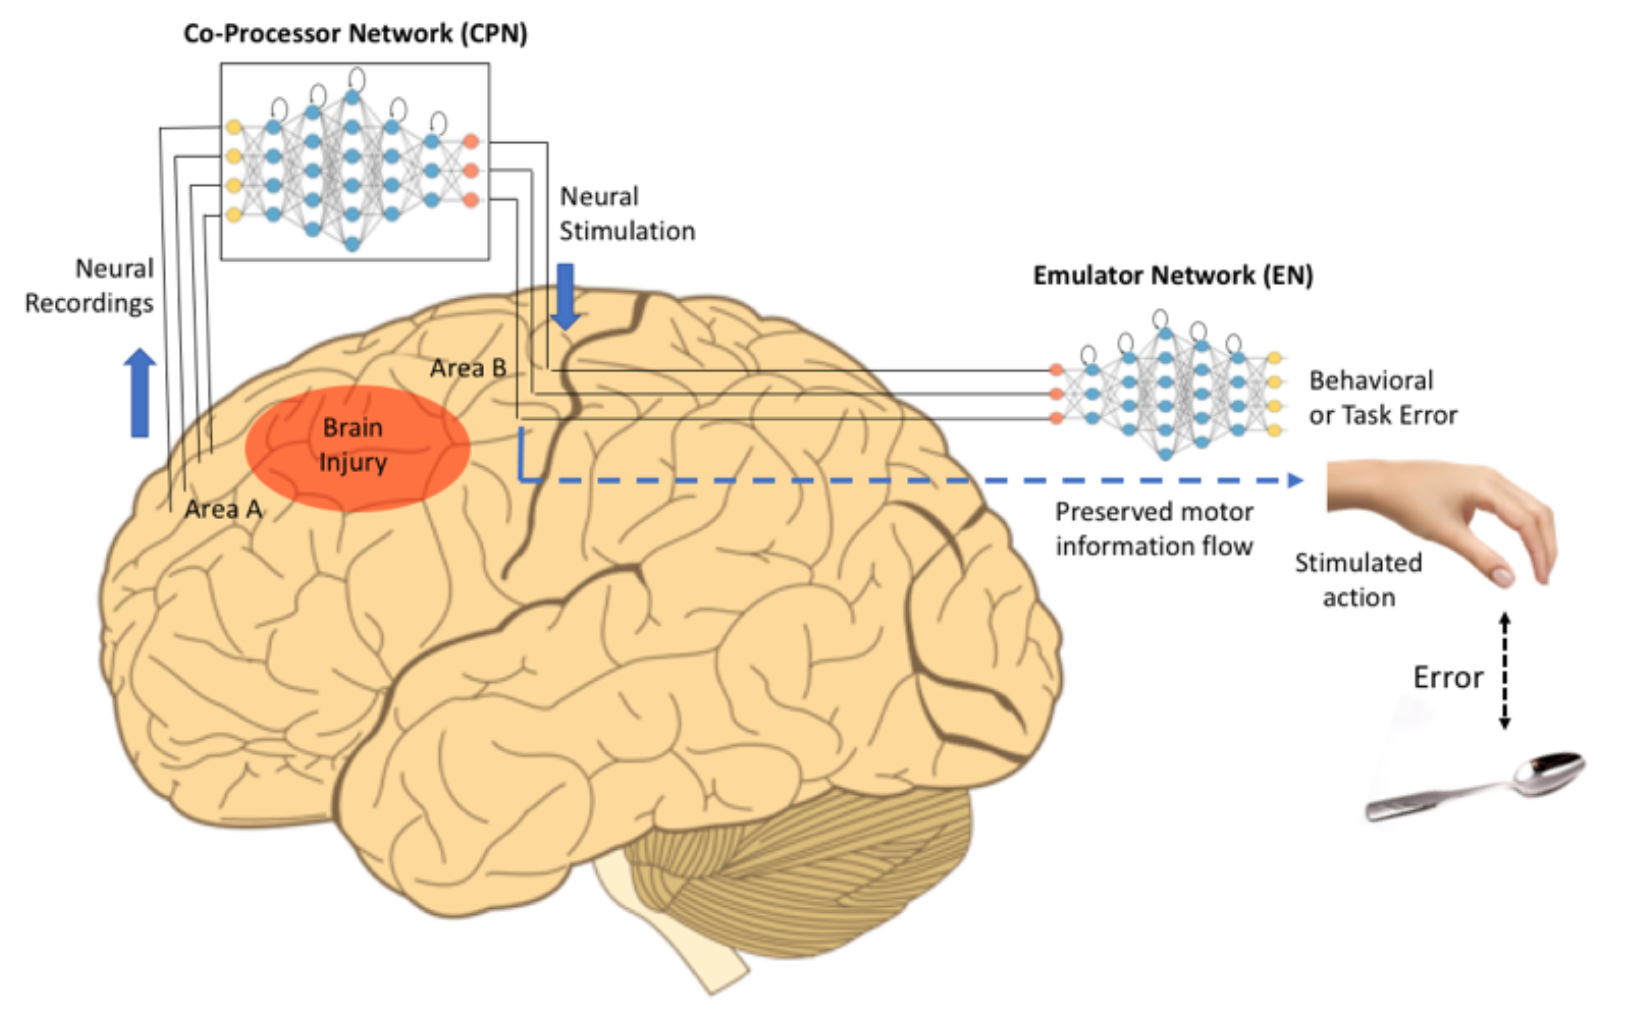
\includegraphics[width=\textwidth]{weill_arch.png}
\caption{Using a co-processor to drive external task performance after a traumatic brain injury}
\centering
\label{fig:weill}
\end{figure}

\subsection{Architecture Overview}
First, we present the architecture of our co-processor design. This design aims to solve two
fundamental challenges in using neural stimulation to improve external task performance.
First, neural networks exhibit long-running and nonlinear dynamics, necessitating
the need for a stimulation agent to account for far-distant effects of the stimulation it
applies. Second, with neurologically complex tasks, such as grasping, the mapping between
neural activity as-measured and the external task cannot be determined \textit{a priori}.
As a result, the co-processor must somehow learn what stimulation is appropriate for
aiding the user in the external task they are attempting to perform.

Our co-processor attempts to solve these with a pair of artificial neural networks:
\begin{itemize}
	\item A stimulation and neural dynamics model, known as an ``Emulator Network'' (EN). It models the relationship
	      between the stimulation, neural dynamics, and external task. Its purpose is for training the second network.
	\item A stimulation agent, known as the ``co-processor network'' (CPN), which maps neural activity, and possibly
	      data from external sensors, to stimulation parameters.
\end{itemize}

We co-train the EN and CPN, with the goal of training a CPN whose output stimulation parameters
improve task performance. By continually training both, they adapt to the brain as it changes,
effectively allowing for brain-stimulator co-adaptation. The EN is a tool for training the CPN,
giving us a way to backpropagate task error to the CPN. It outputs task-relevant
metrics - a prediction of muscle velocities in our case - given measurements of neural
activity, and the stimulation parameters output from the CPN. If the EN is trained in a
particular way, and to a sufficient level of precision, it can be used as a function
approximator relating stimulation and a task, and do so in a way that allows us to train
the CPN with it. When training the CPN, we in-effect treat the EN's output as the true
task performance, or a related metric, and then backpropagate the loss defined in terms
of that metric in order to train the CPN. See Fig. \ref{fig:weill}. We will illustrate the details
of the training algorithm below.

In our present demonstration, the EN is constituted as a single layer, fully connected,
long short-term memory (LSTM) recurrent neural network (RNN), with hyperbolic tangent ($tanh$)
activations, and a linear readout. The general notion of a co-processor does
not require this precise architecture, but for our example, we found that the LSTM
approach allows the network to continuously adapt to long-running dependencies in
the simulated neural dynamics, far better than a vanilla RNN. The CPN is constituted
as an almost identical network, though with a different dimensionality, as we explain
below. There is no strict requirement for the EN and CPN to be so similar, but we
found this simple architecture to work well in our example.

Note that the EN effectively constitutes a stimulation model. However, in the case that
a co-processor attempts to optimize for task performance, as opposed to neural
activity directly, the stimulation model predicts the effect of stimulation and neural
dynamics on task performance, rather than modeling and predicting the neural response
to stimulation alone. This provides the key functionality needed to train the CPN.

We initially attempted an EN architecture using vanilla RNN cells, with a nonlinearity.
This approach resembles the common linear time-invariant state space model of
stimulation, as in e.g. Yang et al. \cite{shanechi.stimmodel}, though it additionally
incorporates a nonlinearity. That approach has the benefit of being simple, and familiar.
We found, however, that the linear approach, as well as the related vanilla RNN
approach with nonlinearities added, was not sufficiently expressive of long-term
dependencies, such that the co-processor was capable of learning well.

Separately, nonlinear LSTM models have also been applied to modeling natural
neural networks, such as use in predicting local field potentials
\cite{kim.lstm}, and for stimulation modeling \cite{guclu.lstm}.
LSTM cells are designed to better capture the relevant aspects of
long-running network dynamics. We found that LSTM cells were crucial for
enabling our co-processor to learn the long-running dynamics of the network
it was stimulating, and we use them as a result.

\subsection{Simulation Overview}
We demonstrate our approach here using a simulated grasping circuit.
A detailed simulation such as this allows us to explore some of the critical
architectural details and training algorithms for a co-processor of this type.
By first doing such exploration in simulation, we are able to rapidly and
cheaply iterate on our design, prior to any \textit{in vivo} experiments.
For the simulation to be admissible, we need to ensure it has some
properties that allow it to strongly indicate if our design is improving in
a direction that will later allow for real deployments. Otherwise, our
design may be adapting to the pecularities of the simulation, without
becoming more useful.

An example of such a simulation approach is Dura-Bernal et al. \cite{bernal.sim}. In this work, the
authors use a simulated spiking neural network to train a stimulation agent.
Their stimulation agent sought to restore the network's
control of a simulated arm, to reach a target, after a simulated lesion was applied,
much like the work here.  As the authors point out, we have a limited ability to
probe a neural circuit \textit{in vivo} in order to perform learning. As a result,
we first need to design our approach through the use of an admissible simulation.
The authors in this case simulated lesions by effectively removing parts of their
simulated network, or by cutting connections between parts of the network.
Here, we use an established design for an artificial neural circuit which
performs a grasping task, whose architecture and training methods were designed
specifically to result in naturalistic dynamics.

The simulated circuit, from Michaels et al. \cite{michaels.mrnn}, was trained
to resemble the grasping circuits of monkey subjects engaged in a delayed reach-to-grasp task.
Its design draws on a body of literature focused on architectures and training methods for RNNs which
seek to create artificial neural circuits that have activation dynamics similar to natural circuits,
including delayed grasping tasks \cite{susillo.mrnn}. The Michaels circuit consists of a
``modular'' vanilla RNN (mRNN), and a linear readout layer. Each ``module'' consists of 100 vanilla
RNN neurons, with a nonlinearity applied on the outputs. The modules are internally fully connected,
and are connected to each other sparsely (10\% connectivity). The inputs are visual features
intended to capture the view the monkeys had during the task, specifically VGGNet features \cite{simonyan.vgg},
from 3D renderings of the same objects which the monkeys grasped. The outputs are muscle length
velocities for the shoulder, arm, and hand of the monkey during the trial. The natural
velocities were captured with a motion capturing glove, and the artificial neural network
was trained to recapitulate those grasping motions. Data and trained models from this work
were supplied to us by the lead author Jonathan Michaels, for the purpose of our present
simulation. We re-implemented his model's logic in PyTorch, and loaded his trained parameters
into it, for one of his subjects, arbitrarily chosen. See Fig. \ref{fig:michaels}.

\begin{figure}
	\centering
	\begin{subfigure}[c]{0.69\textwidth}
		\centering
		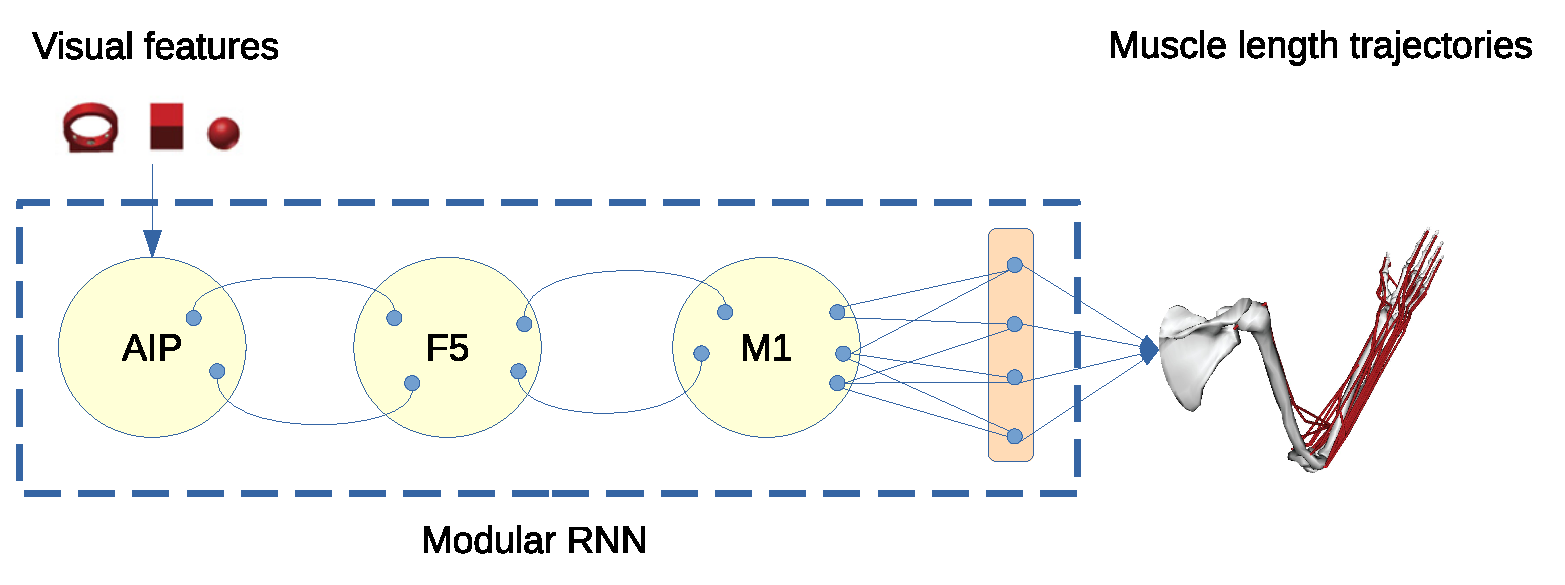
\includegraphics[width=\textwidth]{michaels.eps}
		\caption{Michaels Modular RNN (mRNN), a simulated grasping circuit. The emergent dynamics of the
		three modules correspond well to natural neural activity measured from primate AIP, F5, M1 regions,
		respectively, from the same task. Visual (VGGNet) features forward propagate through the
		network, conditioning the grasp for the object of the particular size, shape, and location.}
	\end{subfigure}
	\hfill
	\begin{subfigure}[c]{0.30\textwidth}
		\centering
		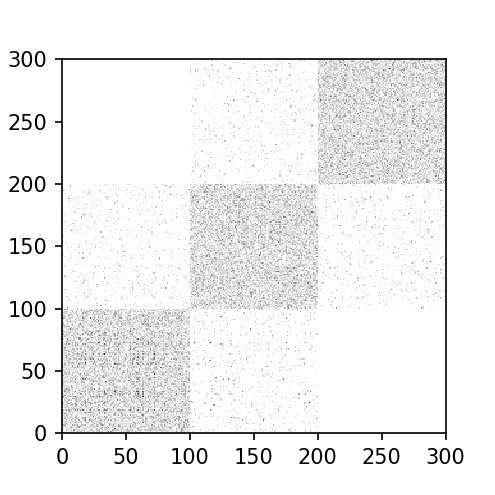
\includegraphics[width=\textwidth]{mRNN_J.png}
		\caption{Connectivity matrix $J$. Note the within-module connections
		(on the diagonal) are fully connected, and connections to adjacent
		modules are sparse $10\%$.}
	\end{subfigure}
	\hfill
\caption{Architecture of the Michaels mRNN}
\label{fig:michaels}
\end{figure}

The design of the circuit is intended to resemble a vision-to-grasp pipeline, essentially
representing the visual processing needed to reach the hand to the appropriate position for
the grasp, and to form the hand properly for grasping the particular shape of object. The
emergent dynamics of the artificial network's ``modules'', once trained, correspond roughly
to the AIP, F5, and M1 portions of the monkey subjects' brains. `Correspond' here, notably,
refers to the fact that the activity of the module receiving the visual inputs resembles
the AIP activity of the monkey subject from the same trials. Likewise, the second and
third modules resemble the natural activity from the monkey's F5 and M1 regions, respectively.
The emergent network dynamics show a number of other correspondences to the monkeys' natural
brain activity as well, as detailed in the paper.

Importantly, the simulated circuit's activity shows a relatively clear separation of the
object shapes. That is - the visual information input to the network that differentiates
one trial from another is leveraged by the circuit to properly condition
the hand shape trajectory for grasping the object of that trial's particular shape, size, and
location. The visual information forward-propagates through the network, through successive
processing steps, where it is eventually leveraged to recapitulate the grasp appropriate
for the object represented by the input visual features. It follows, then, that the classes
are separable in some way by observing the distinct ways that the mRNN is activated by the
classes' corresponding visual inputs. As we will note below: in the absense of this
visual information forward propagating, the circuit can at-best learn a loss-minimizing grasp,
stereotyped across all object sizes and shapes. Such a grasp bears some resemblance to all
grasps the given monkey performed, due to all trials being a reach-to-grasp preceded by a
waiting period, but performance suffers drastically.

Clearly, training and deploying a neural co-processor in a true brain involves challenges we
don't capture with this simulation. This simulation does not constitute evidence
that our method will, for example, immediately translate to true restoration of fine-grained
control for individual fingers of a stroke patient. One clear challenge with doing so would
be the sheer dimensionality of natural brain dynamics, and how that compares to the resolution
of stimulation the co-processor can learn to apply. There exists a clear mismatch between
the dimensionality of the underlying problem, sensor and stimulator technologies, and the
amount of training data which can reasonably be collected to train a closed-loop neural
controller. We argue that while this fact clearly creates a challenge for learning-based
closed-loop stimulation, that nevertheless the insights we generate through this
simulation are likely to be applicable. In the Discussion below, we will explore how
those insights are likely to lead to initial demonstrations of the co-processor approach
on lower dimensional problems. As we show next, the simulation exhibits a number of
properties that reflect a real world application, which our co-processor design must
contend with.

\subsubsection{Simulated lesions cause real world failure modes}
Simulating a brain lesion in terms of this artificial network results in error
modes that resemble a some natural lesions of a primate brain. For example, if we
alter the network by zeroing the outputs of some of the first (input, or AIP) module's neurons,
the reaching motion generally succeeds, but the finger muscle velocities show a high degree
of error - effectively implying that the subject can somewhat reach to grasp, but cannot form a
grasp appropriate for the object. That suggests that losing a portion of the cortical
machinery needed to translate or forward-propagate object shape information
to movement-related cortex can result in a reduced ability to form the hand properly for
the grasp, though positioning of the hand may still roughly succeed. Muscle spasticity of
the hand is also a common symptom of certain strokes in primates, and indeed many who
suffer from it are still able to position their hand, even while being unable to form
it properly for a grasp \cite{khanna.openloop}. In that sense, the error mode of this
simulated lesion closely resembles natural stroke symptoms. However, the simulation is not
intended to constitute a physical model of a lesion, i.e. to directly explain the
connection between hand spasticity and the lesion.

Conversely, if we lesion of a portion of the output module of the Michaels mRNN, roughly
corresponding to M1, we see a more wholesale loss of movement, affecting even the
ability to reach for the grasp. Finally, if we ``disconnect'' communications between the
F5 and M1 modules, we see a failure similar to an AIP lesion: movement is generally
achieved, but we see a disproportionate impact on hand pose.
See Fig. \ref{fig:lesion} for examples.

\begin{figure}[h]
	\centering
	\begin{subfigure}[c]{0.62\textwidth}
	    \centering
	    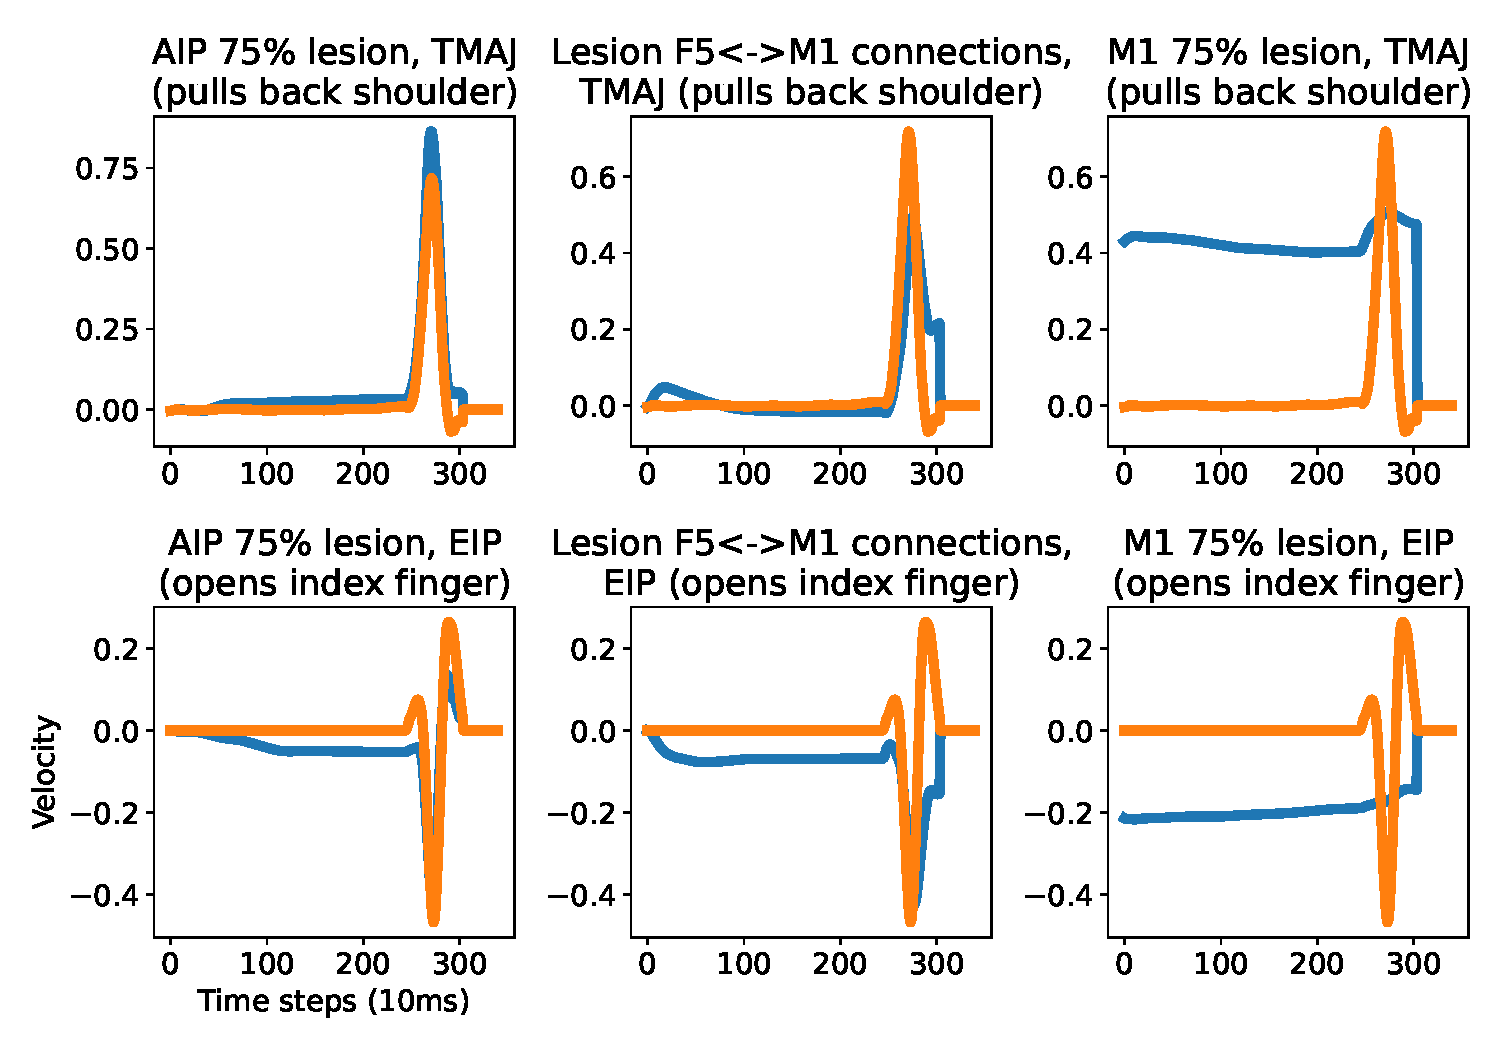
\includegraphics[width=\textwidth]{lesion_trajs.pdf}
	    \caption{Example muscle trajectories during a single trial, for one hand and shoulder muscle}
	\end{subfigure}
	\hfill
	\begin{subfigure}[c]{0.32\textwidth}
	    \centering
	    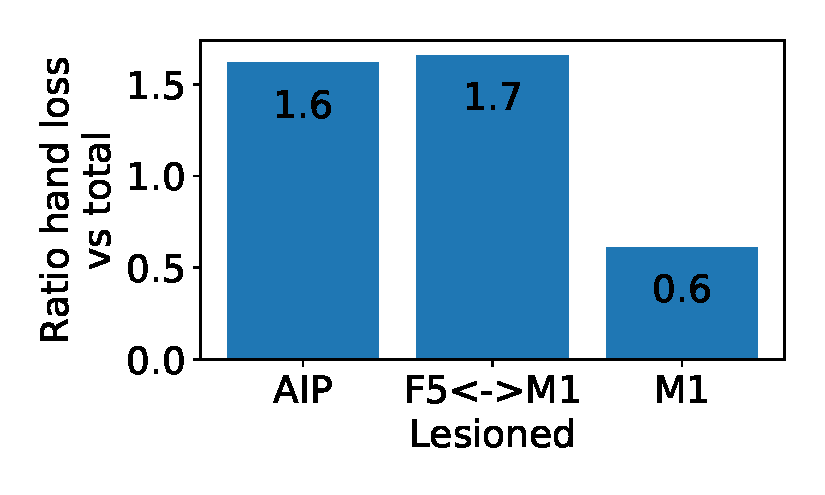
\includegraphics[width=\textwidth]{lesion_hand.pdf}
	    \caption{Ratio of hand muscle MSE losses vs. overall MSE losses, for different lesion types}
	\end{subfigure}
	\hfill
	\caption{Lesion designs which prevent forward propagation of object shape information
	         differentially impact hand pose. Loss here is an L2 distance
		 measured relative to the circuit's trajectories prior to the lesion.}
	\label{fig:lesion}
\end{figure}

The co-processor's task in our simulation will be identifying the appropriate information,
read from the mRNN's activations, for conditioning the stimulation. The co-processor seeks
to effectively bridge across the lesion, forward propagating the object shape and task
structyure information, indirectly, through the use of stimulation.

In our experiments below, we demonstrate our co-processor design on three types of
simulated lesions:
\begin{itemize}
	\item \textbf{Output-based (AIP):} we force the output of some proportion of ``AIP''
	      neurons to zero, effectively removing them from the network. This results in a
	      loss of object shape information until the brain co-adapts to the lesion.
	\item \textbf{Connection-based:} we prevent the propagation of
	      information between the ``F5'' and ``M1'' modules, effectively representing a
	      severing of the connections between the two. Note that the sparse connections
	      between them run both directions, and we are lesioning both.
	\item \textbf{Output-based (M1):} we force the output of some proportion of ``M1''
	      neurons to zero, causing a more holisitic loss of movement. Here, the lesion
	      may make it impossible for the co-processor to find a solution, but some
	      recovery may be possible.
\end{itemize}

\subsubsection{Simulated network exhibits long running dynamics}
Just as the co-processor must adapt to the lesion, it must also adapt to the dynamics of
the network it is stimulating. Natural neural networks as well as our simulated network
exhibit long running dynamics, which our CPN and EN must account for in their learning.
A perturbation of a network (i.e. due to stimulation) will cause changes in neuron
activations long after the stimulation is applied, sometimes far from the site of
stimulation. Our simulated grasping circuit exhibits the same behavior.

To illustrate this, suppose we applied a small, one-time, instantaneous perturbation
of the hidden state of 10 randomly chosen neurons in the output (M1) module at some point
in time during a trial. If we repeat that experiment many times, we can see what the
distribution of long- running effects tends to look like.

In Fig. \ref{fig:dynamics} we can see that even a single, one-time perturbation in
the network has effects dozens of time steps later. Our co-processor will need to
account for these dynamics, since stimulation is intended to cause perturbations
in a network. As we will show in the next subsection, the problem the co-processor faces
is in-fact even harder than this, due to a stimulation model that includes both
spatial and temporal smoothing.

\begin{figure}[h]
	\centering
	\begin{subfigure}[c]{0.48\textwidth}
	    \centering
	    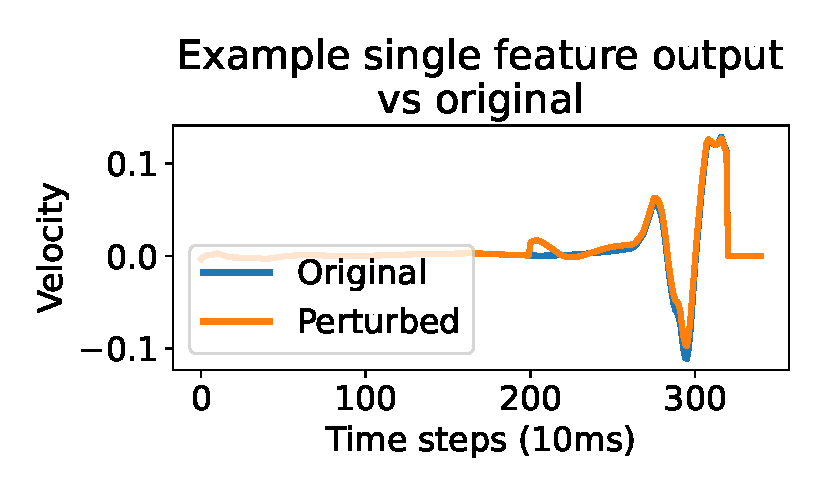
\includegraphics[width=\textwidth]{perturbe_single.pdf}
	    \caption{Example trial}
	\end{subfigure}
	\hfill
	\begin{subfigure}[c]{0.48\textwidth}
	    \centering
	    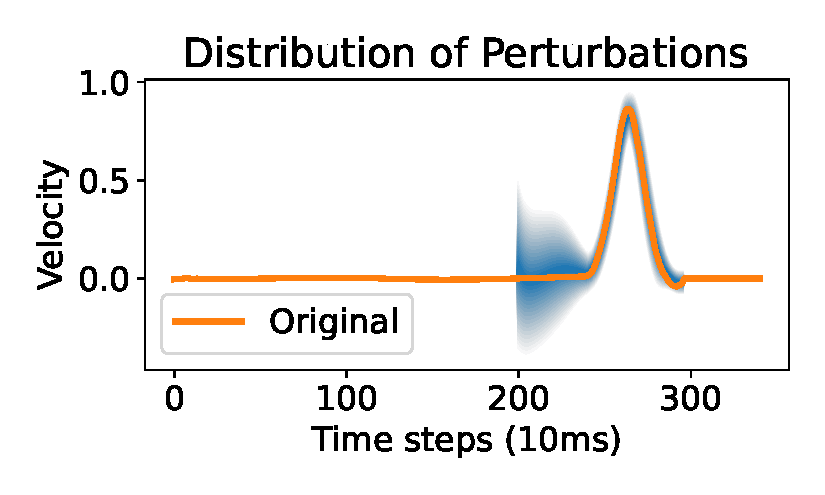
\includegraphics[width=\textwidth]{perturbe_dist.pdf}
	    \caption{Distribution of effects across n=1000 samples}
	\end{subfigure}
	\hfill
	\caption{Instantaneous perturbations of a random sample (n=10) of M1
	         neurons at time t=200 results in long-running effects on output.}
	\label{fig:dynamics}
\end{figure}

\subsubsection{Stimulation model}

\begin{figure}[h]
	\begin{subfigure}[c]{0.45\textwidth}
		\centering
		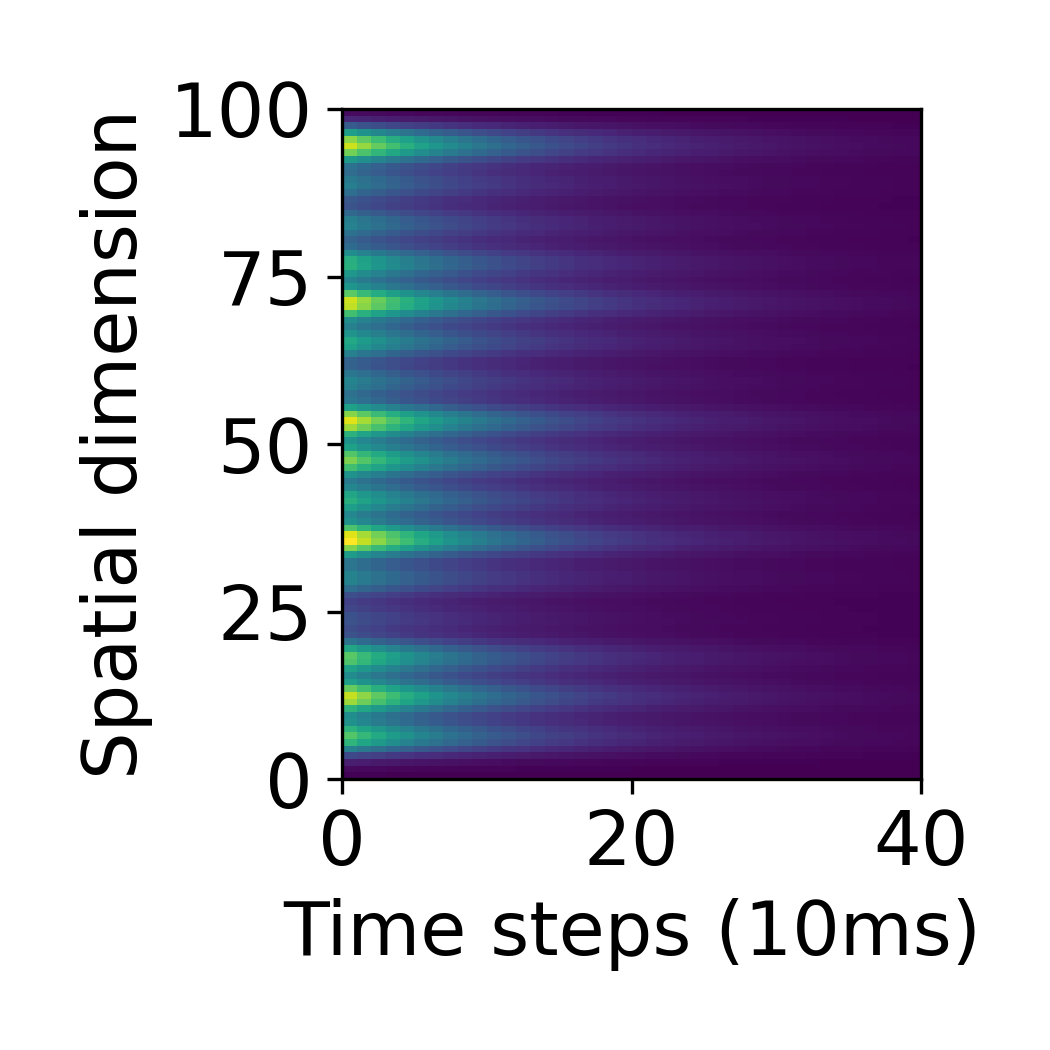
\includegraphics[width=\textwidth]{stim_single.png}
		\caption{$\sigma=1.875$}
	\end{subfigure}
	\hfill
	\begin{subfigure}[c]{0.45\textwidth}
		\centering
		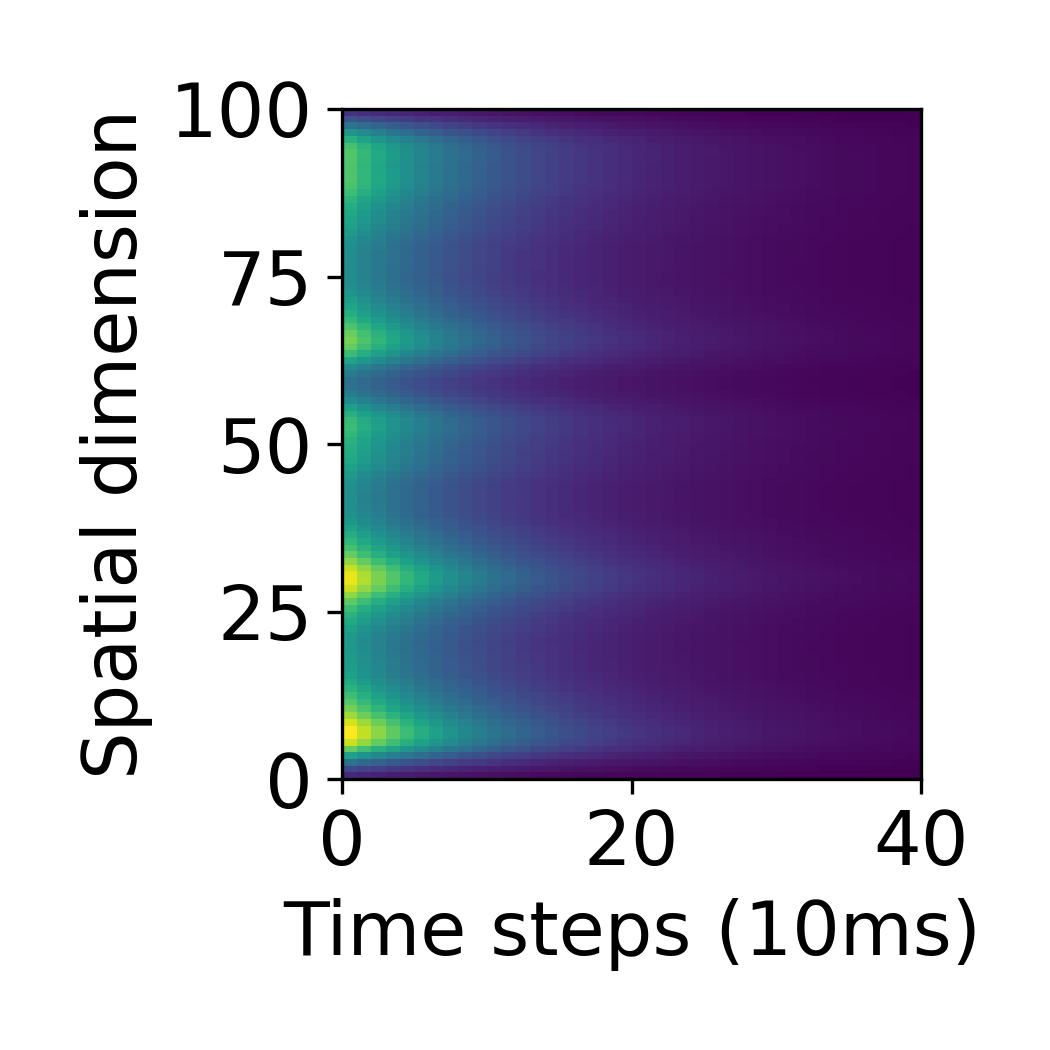
\includegraphics[width=\textwidth]{stim_single2.png}
		\caption{$\sigma=2.875$}
	\end{subfigure}

	\caption{Spatial and temporal smoothing of a single 16 dimensional,
	         randomized $\theta$, onto 100 simulated neurons.
		 Color values indicate the magnitude of the value summed into
		 each neuron's hidden state in that time step. After $t=0$,
		 $\theta$ is the zero vector.}
	\label{fig:stim_single}
\end{figure}

In order to inject another aspect of realism into our simulation, we subject
the co-processor to a stimulation model, rather than allowing it to directly
influence the hidden state of the simulated network's neurons. Our stimulation
model includes aspects of both spatial and temporal smoothing.

The intent with this approach is not to create a realistic biophysical model. The
mRNN model does not contain sufficient information to arrange the neurons in a
simulated space, and to simulate how that may change the effects of stimulation.
Instead, our stimulation model is merely attempting to make the co-processor's task
more realistic, in the sense that it cannot precisely set the hidden state of every
neuron, instantaneously and in each time step. Any stimulation it applies will diffuse
across ``space'' and time.

In our experiments, we stimulate only the output module, since this co-processor's
purpose is to improve external task performance, which it is able to do with
only stimulation of the output module of the network. It is conceivable that
a co-processor could stimulate other areas of the brain to improve task performance
downstream, or to probe the brain to better reveal the user's intent (i.e. object
shape), but we did not explore those possibilities in this paper.

The stimulation function $S$ receives as inputs the stimulation parameters $\theta$
provided by the CPN, which it accumulates in an internal memory. Each time step,
it outputs a modifier to the internal states of all neurons in the output module,
based on the current state of memory. That memory allows
the stimulation function to perform temporal smoothing. Specifically, we used a
simple exponential decay model where the function reads its current state of memory,
sums in the new parameters, and then decays each memory element towards $0.0$ at some
rate. Roughly speaking, this design intends to approximate the notion of dissipation: the
effect of stimulation is not instantaneous, but rather decays with time, as charge
dissipates into the surrounding area.

Likewise, the stimulation function maps the relatively low dimensional stimulation
parameter vector $\theta$ onto the M1 cells which it stimulates. In our experiments,
our stimulation parameters $\theta$ had 16 dimensions, which we found was
sufficient to allow significant improvement in task performance. The stimulation
function uses a simple Gaussian smoothing to map those parameters onto the simulated
M1 neurons. Each parameter represents, in a sense, an electrode located along a single
spatial dimension, whose stimulation affects the neurons in its vicinity more than
it affects others, according to each neuron's Mahalanobis distance from it. The neurons
are aligned along that dimension arbitrarily. We fix the width of the Gaussians
arbitrarily to $\sigma=1.75$. We are not aware of a principled way of picking this
value, and clearly if we set it to extreme values, it makes our simulation less useful.
For example, if it is set to an extreme high value, the stimulation is effectively
lower dimensional, resulting in a model corresponding to a stimulation technology that
is inappropriately low resolution for our task, for example epidural stimulation.
However, we cannot conclude much from these experiments, because this simulation does
not constitute a biophysical model, where we can identify some realistic value. The
purpose of this smoothing technique is only to make the co-processor's job harder in
the simple sense that it cannot target neurons individually.
As a result, we set it to a moderate, balanced value, and don't vary it.

Thus, the governing equations of the stimulation become:

\begin{equation}
\alpha_{t} = \tau\alpha_{t-1} + \theta_{t-1}
\end{equation}
\begin{equation}
s_{t} = C(\alpha_{t})
\end{equation}

\begin{itemize}
	\item $\alpha$: the 16 dimensional internal activation, or memory
        of our stimulation
	\item $\tau$: our decay rate, which we set arbitrarily to $0.7$
	\item $C$: a precalculated $100 x 16$ matrix which provides our
	Gaussian smoothing
	\item $s_{t}$: the stimulation we apply to each neuron at the
	given time step.
\end{itemize}

The governing equations of the simulated network then become:

\begin{equation}
x_{t+1} = Jx_{t} + Iv_{t} + s_{t} + b
\end{equation}
\begin{equation}
a_{t} = tanh(x_{t})
\end{equation}
\begin{equation}
y_{t} = La_{t} + l
\end{equation}

\begin{itemize}
	\item $x$: the hidden state of each neuron
	\item $J$: the recurrence weight matrix
	\item $I$: the input response matrix
	\item $b$: the neuron activation bias
	\item $L$, $l$: the parameters of the linear readout
	\item $y$: the output of the network
\end{itemize}

See Fig. \ref{fig:stim_single} for a visual depiction of an example where
$\theta$ is non-zero at $t=0$, and zero for all other times, in order to see how
stimulation is applied across space and time. In Fig. \ref{fig:stim_and_obs},
we see stimulation applied during the simulation, in a real trial. In this case,
the trial is one where $50\%$ of M1 neurons are lesioned to have zero output.
Observations of the network's hidden state (explained in the next section) are taken
from the first two modules, and stimulation is applied to the last module. This fact
is intended to capture the difficulties with observing the same region that you are
stimulating, due to stimulation artifacts. The trial we show depicts stimulation
supplied by a highly trained co-processor, where task performance has been
largely restored. We explain this experiment in more detail below.

\begin{figure}[h]
	\centering
	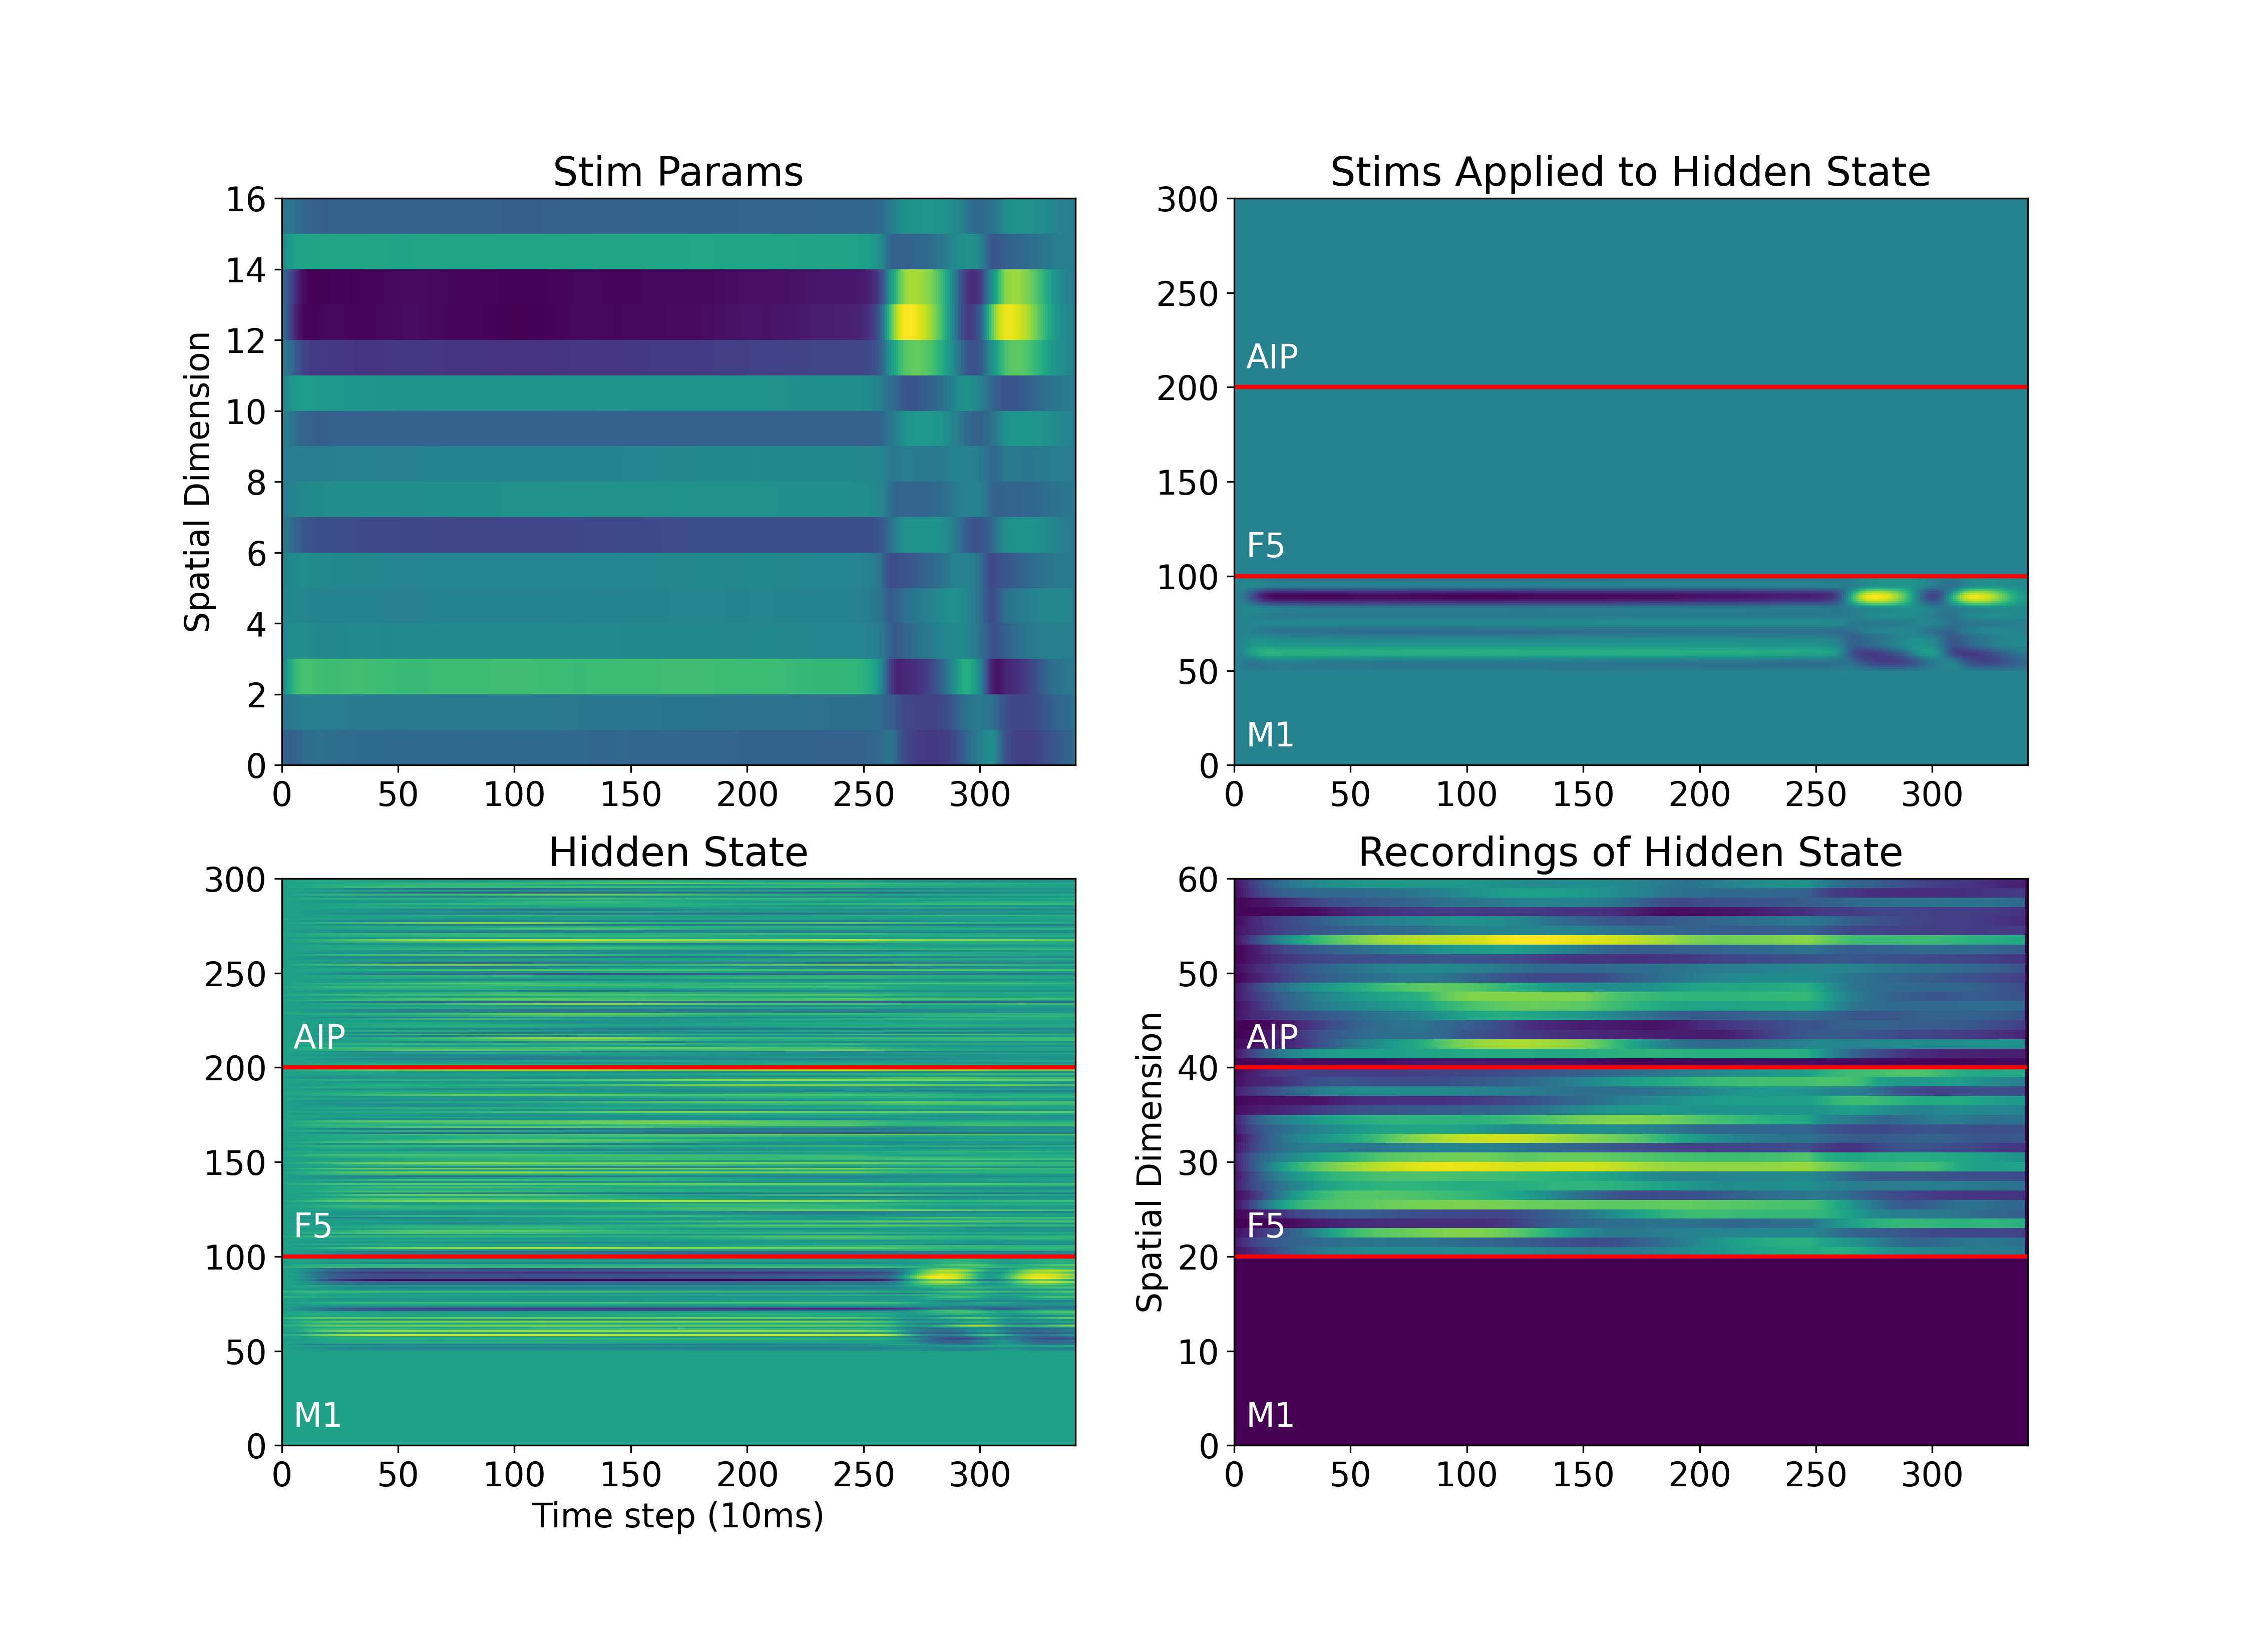
\includegraphics[width=\textwidth]{stim_and_obs.png}
	\caption{Example of stimulation and observation for a single trial. Here, M1
	has been lesioned 50\%, as seen in the zero (light blue) hidden states. We
	gather observations only from the AIP and F5 modules, as we explain in
	Section \ref{sec:experiments}. Stimulation is applied to M1, to drive the
	network output.}
	\label{fig:stim_and_obs}
\end{figure}

\subsubsection{Observation model}
Our observation model likewise relies on a notion of electrodes spread along
a single spatial dimension. As with stimulation, this is not intended to
capture true physical relationships between neurons and electrodes, but
rather to act as a dimensionality reduction that isn't designed to specifically
favor task success, such as PCA. We treat the neurons of each module as
occupying their own space, with 20 electrodes arrayed along each.

We use a similar Gaussian-based approach as with stimulation, but in this
case our approach looks much like a Gaussian convolution, where the Gaussian
kernel is centered at each electrode position. Each `electrode' is read out
as a weighted average of all neurons in the given module, with weights being
provided by the Gaussian kernel. As above, refer to Fig. \ref{fig:stim_and_obs}
for a visual example.

\subsubsection{Brain co-adaptation}
To demonstrate the co-processor's ability to adapt to the non-stationarity
of the brain, we also change the brain throughout the co-processor's training.
Specifically, we simulate the brain's co-adaptation with the stimulation
to cooperatively solve the problem, as the stimulation is also changing
through the CPN's training.

We achieve this through a simple error backpropagation, using PyTorch's
implementation of the $Adam$ optimizer. With each trial, task loss is
calculated and backpropagated into the mRNN, allowing it to adapt to
the fact it receives stimulation. The learning rate for the optimizer
is set arbitrarily to a relatively low rate of $1e-7$. The learning
rate was not chosen in a principled way, since we are not aware of a
principled way of choosing it. However, we reason that it should be
lower than the co-processor by orders of magnitude due
to the rapidity with which an ANN can be retrained.

\subsubsection{Simulating recovery prior to co-processor use}
We sought to additonally re-train the mRNN after applying the lesion in
order to simulate stroke recovery. For simulated lesions which zero the outputs
of neurons, the mRNN is, unfortunately, not an appropriate model.
We know that strokes can cause damage from which the subject, in many cases,
cannot recover. The mRNN model has sufficient redundancy built into it that
lesioning the outputs of large numbers of neurons leaves enough remaining
degrees of freedom that a nearly full recovery can occur, unless so many
neurons are lesioned that no stimulation could be effective.

We can, however, simulate pre-recovery in the case of a lesion that excludes
communication between the F5 and M1 modules. In that case, object shape information
cannot propagate forward in the network, in order to condition the hand for
grasping. The mRNN can, in pre-recovery, learn a stereotyped grasp, at which
point the co-processor's job will be to forward-propagate that information.
We explore this in one of our experiments, explained below.

\subsection{Training Algorithm}
In all experiments, training the co-processor requires a careful interleaving of
EN and CPN training epochs. EN training epochs concentrate on updating the EN,
based on observations of the effect of stimulation on the simulated network's output.
The loss function when training the EN is the mean squared error (MSE) loss between the
actual and predicted output of the mRNN (i.e. muscle velocities). We then use the EN
to train the CPN during the CPN training epochs. During that time, we backpropagate
the MSE loss between the EN's predicted output, and target output, to the CPN. In
other words: we treat the EN output as a proxy to the true brain, allowing us
to train the CPN, since we have no way to ``backpropagate through the brain'' itself.
See Fig. \ref{fig:training}.

\begin{figure}
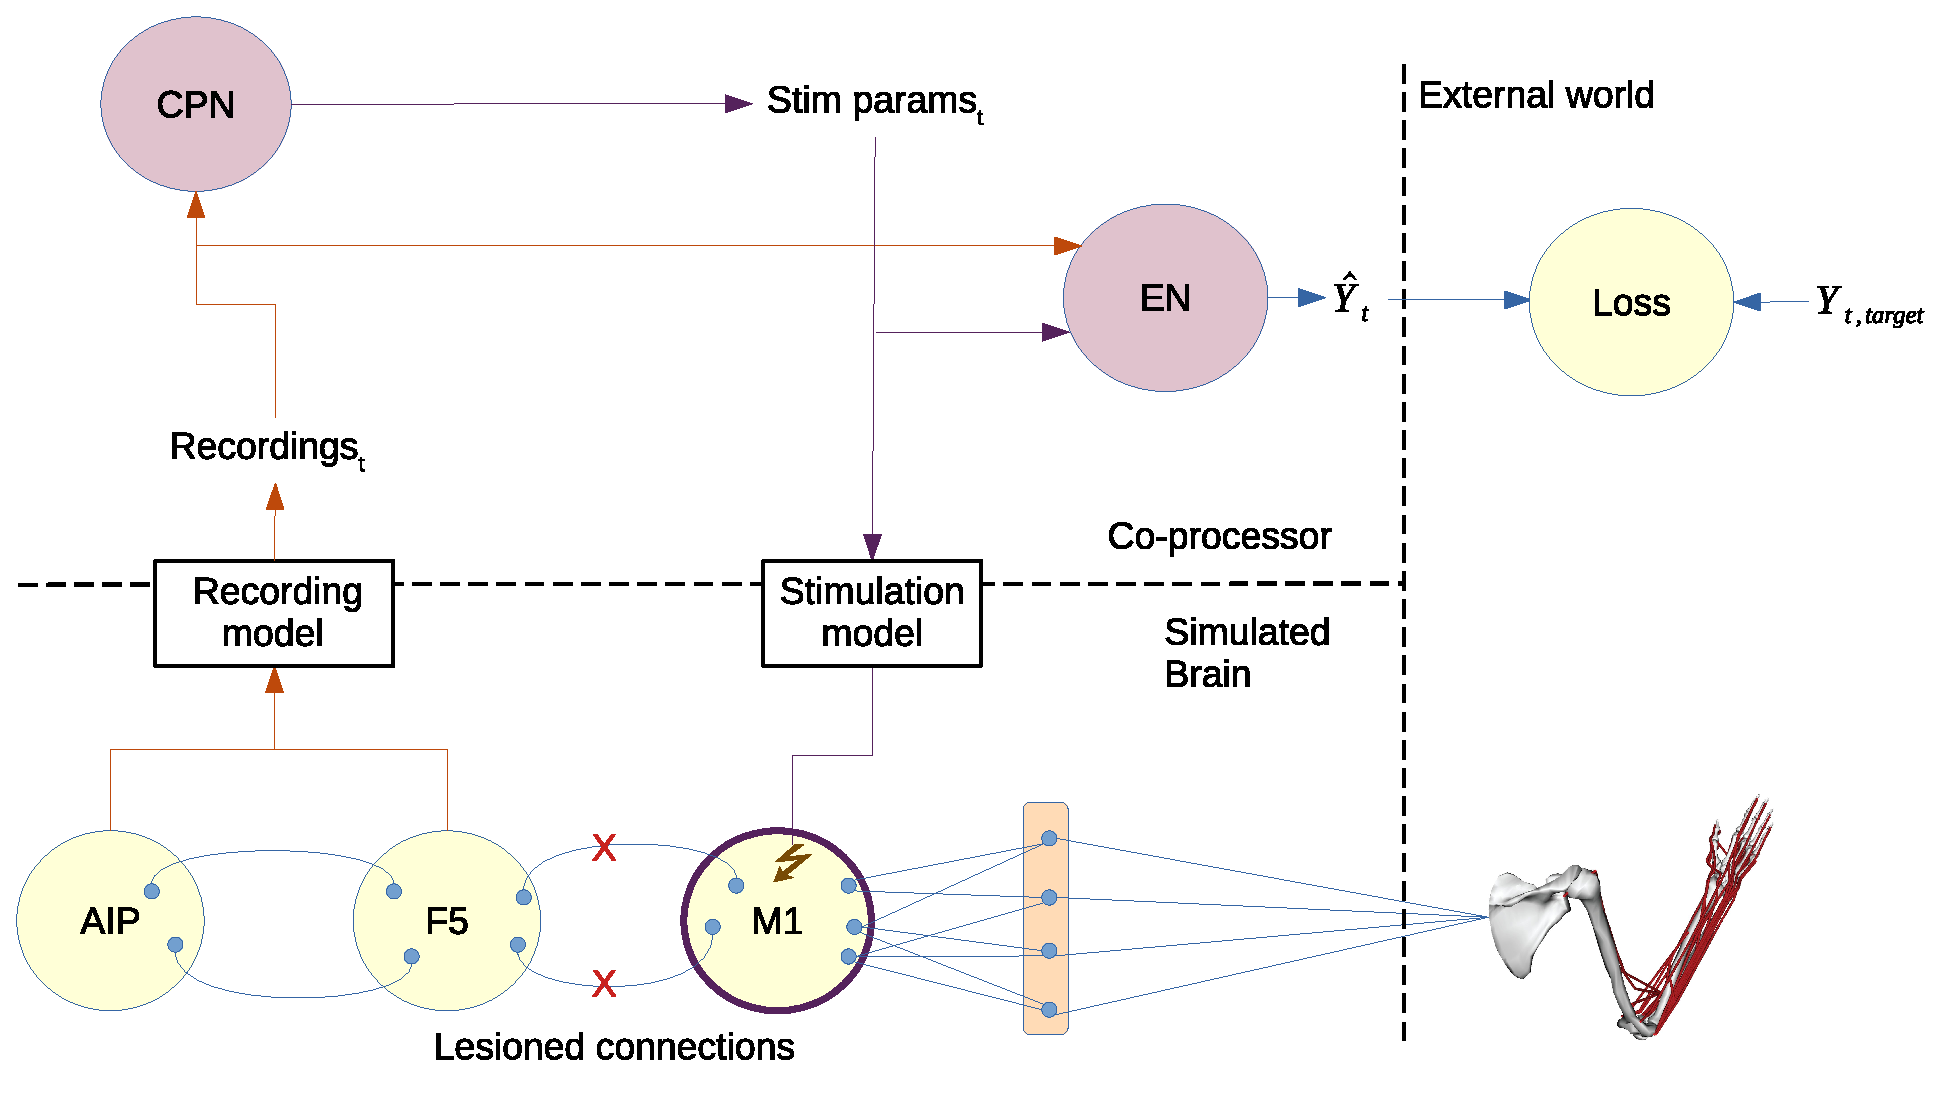
\includegraphics[width=\textwidth]{cpn_michaels_arch_labeled.eps}
\caption{Experiment architecture overview}
\centering
\label{fig:exp_overview}
\end{figure}

\begin{figure}
	\centering
	\begin{subfigure}[c]{0.48\textwidth}
		\centering
		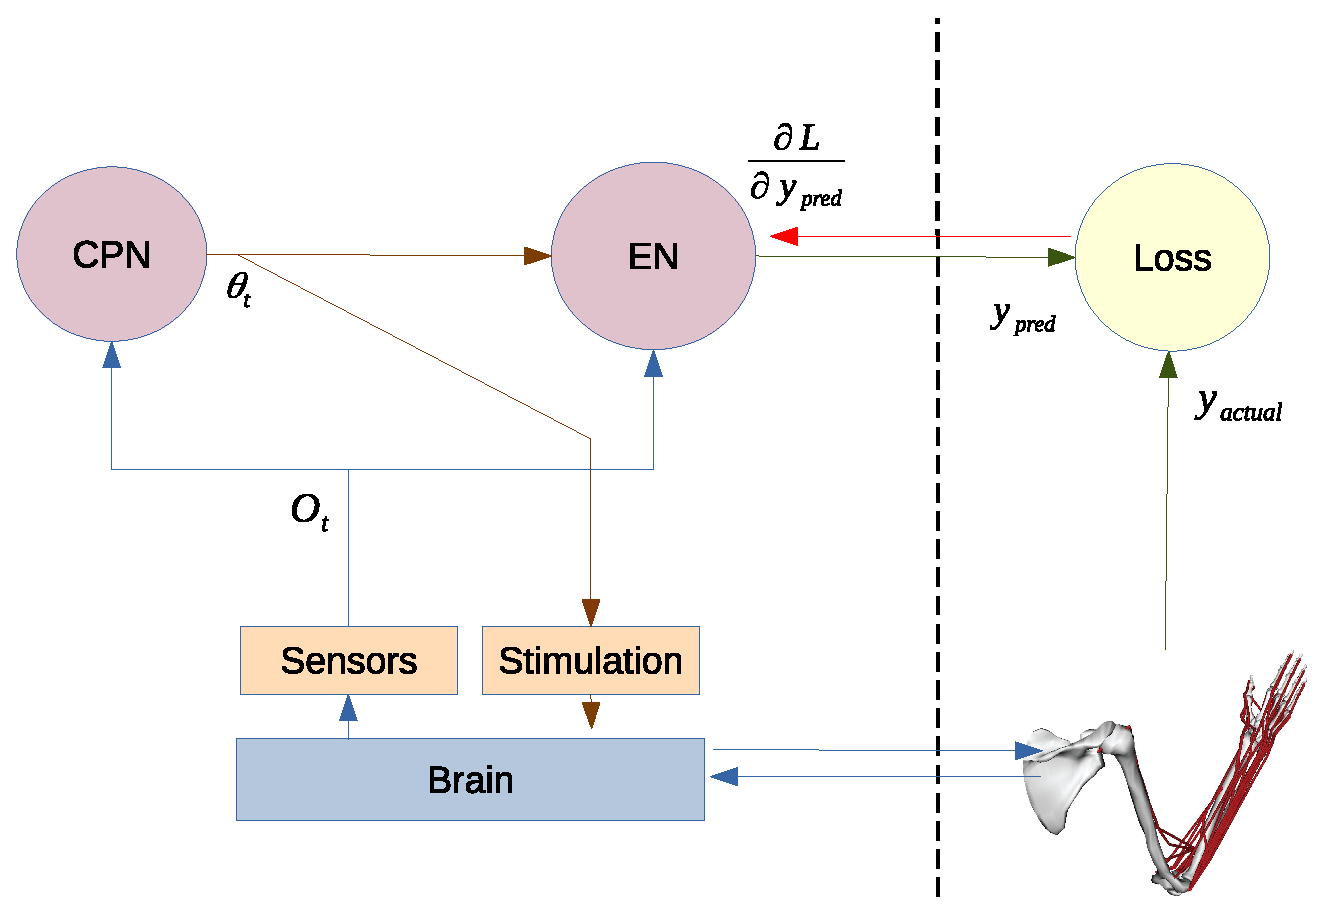
\includegraphics[width=\textwidth]{backprop_en.eps}
		\caption{EN training phase: backpropagate actual vs predicted}
	\end{subfigure}
	\hfill
	\begin{subfigure}[c]{0.48\textwidth}
		\centering
		\includegraphics[width=\textwidth]{backprop_cpn.eps}
		\caption{CPN training phase: backpropagate actual vs target MSE loss, via EN, to CPN. This effectively treats the EN output as the actual, and thus the EN must be trained first.}
	\end{subfigure}
	\hfill
\caption{Two Phase Training Regime}
\label{fig:training}
\end{figure}

\subsubsection{EN training}
For the EN to be useful, it must accurately predict the effect of stimulation
produced by the CPN. In addition to that, backpropagating through it must yield
gradients which train the CPN to output more useful stimulation. We discovered that
this latter property does not occur simply by virtue of the former.
We have found that an EN can be trained to high levels of predictive power, even
on random stimulation, and to orders of magnitude lower loss than the task loss,
while at the same time backpropagation through it yields gradients which are not
useful for training the CPN. As a result, if the EN is not trained in specific ways,
the CPN exhibits unstable training. We have thus far been unable to discover a way
to measure and optimize for this second property directly, though pursuing it may be a
fruitful subject of future applied ML research. Instead of attempting to train an EN
directly to exhibit this property, we discovered a training regime that indirectly,
but reliably, makes it occur.

The central concept of our training regime is to provide a carefully chosen variety of
training examples, and to use heavy weight regularization, in order to force
the EN to generalize well to stimulation which it hasn't yet seen. We hypothesize that
the crux of our EN training problem is one of over-fitting: that the EN may be trained
to high predictive power on a set of stimulation examples, but that the effective
dimensionality of the problem it is learning is comparatively quite high, due to both
the dimensionality of our stimulation parameters $\theta$, and the dynamics of the
network being stimulated. As a result, the hypersurface which it fits to the training
examples may exhibit gradients not reflective of reality.

First, and most significantly, we structure the training dataset for each EN training epoch
in a very specific way. Each epoch, we include:
\begin{itemize}
	\item examples using stimulation from the current CPN
	\item examples from a small (100s) collection of CPNs which are copies of the
	      current CPN, with Gaussian-distributed mean-0 noise added to their parameters
	\item examples of white noise stimulation
\end{itemize}
We developed this structure under the belief that we needed to cover a sufficient
variety of examples to prevent overfit, and to do so in a way that emphasizes the neighborhood
in CPN parameter space of the current CPN. We initially attempted to pad our dataset with white
noise examples alone, but that was not sufficient to stabilize CPN training, despite the EN's
ability to reach a high predictive power. Adding in the addition of samples from the parameter
space near the current CPN appears to help ensure that the EN is localized enough to give
useful gradients for that area. As we will explain below, this produces an additional problem
that the EN is too specialized to the local area of CPN parameter space, but we then solve
that problem using EN retraining, interleaved with the CPN training.

After some experimentation, we composed each batch of EN training data in the following way: \\

\begin{tabular}{|l|l|}
\hline
\textbf{Source}                                                                                                                            & \textbf{Proportion of dataset} \\ \hline
Current CPN                                                                                                       & 10\%                           \\ \hline
\begin{tabular}[c]{@{}l@{}}Current CPN with parameter noise\end{tabular} & 60\%                           \\ \hline
White noise stimulation                                                                                                        & 30\%                           \\ \hline
\end{tabular} \\

Additionally, we use PyTorch's $AdamW$ optimizer, which includes an option for weight regularization.
With that, we use a carefully chosen learning rate schedule. Our intuition is to leverage regularization as
one of the standard mitigations for overfit. To converge, the learning rate schedule needs
to be chosen carefully: a relatively high learning rate at first, dropping to a very low rate soon
thereafter. Using too-low or too-high of a learning rate in any phase causes the EN learning
to not converge. EN training proceeds until it reaches a threshold of prediction error, defined as
a fraction of the current CPN's task loss.

\subsubsection{CPN training}
Once an EN is properly trained, CPN training is straightforward. For this phase,
we generate training examples using the current CPN alone. The EN generates predictions of the
effect of those stimulations, and we backpropagate through the EN to generate training gradients
for the CPN. As with the EN, we constitute the dataset with a large random sample of trials from
the original Michaels task. See Fig. \ref{fig:training}.

The choice of learning rate schedule for training the CPN is somewhat important.
The CPN appears to train in two phases. In the first phase, it is largely learning the structure
of the reach-to-grasp task, e.g. that the muscles need to stay still until the reach begins. During
that phase, the learning rate can be quite high. Later, the CPN begins to learn the mapping between
the object shape information observed from the simulated brain, and how that should map onto
stimulation. That phase of the training takes much longer, and requires a learning rate 2-3
orders of magnitude lower than in the first phase. We will cover this in some more detail in
Section \ref{sec:results}.

\subsubsection{Interleaved CPN/EN training, and adapting to non-stationarity}
Having defined the training periods for the EN and CPN, we can define a training
algorithm on the basis of those two. We train the two in alternation, creating
a new EN each time we enter an EN training period. We explored the possibility
of reusing an existing EN by retraining it, for the purpose of training efficiency.
However, we found that retraining an EN was no more fast than training a new one,
and in-fact usually took longer, despite significant experimentation with learning
rates. It is unclear if that fact is an artifact of our simulation, or of the
problem more generally, and so it needs more examination in the future, for the
purpose of training efficiency.

The key remaining challenge is determining when an EN is no longer suitable for training the
current CPN. Expiring an EN at the right time accomplishes two things. First, it ensures
that our current EN is trained properly for the current CPN; without that, the CPN training
will become unstable. Second, expiring the EN is how we adapt our learning to the brain's
non-stationarity. At some point, the brain will have changed sufficiently for our EN to be
out-of-date, and therefore requiring replacement.

We solve this challenge through a simple set of metrics, which, when satisfied, indicate
we need to transition to an EN training period. Our first metric simply captures the EN's
declining predictive power. When the EN's prediction error reaches a point which is
sufficiently above some ratio to the CPN's task loss, we expire the EN immediately.
Second, we expire the EN if CPN loss does not improve (or gets worse) across a sufficient
number of recent training steps. This resembles common stopping conditions in
iterative learning: one stops when learning is no longer improving the model. Together,
these two metrics appear effective in ensuring we expire the EN at the right time.

\subsection{Experiments}
\label{sec:experiments}

Using the simulation described above, we perform several experiments to
demonstrate the co-processor's ability to learn. In each experiment, we apply one
of the three lesion types described above. We additionally vary whether we simulate
brain co-adaptation, in order to understand its impact on the co-processor training.
Finally, we perform one experiment where we attempt to simulate natural recovery from
the lesion, prior to training the co-processor. In sum, our experiments are: \\

\begin{tabular}{|l|l|c|c|}
\hline
\textbf{Index} & \textbf{Lesion}                                           & \multicolumn{1}{l|}{\textbf{\begin{tabular}[c]{@{}l@{}}Simulate\\ co-adaptation?\end{tabular}}} & \multicolumn{1}{l|}{\textbf{\begin{tabular}[c]{@{}l@{}}Simulate\\ pre-recovery?\end{tabular}}} \\ \hline
1              & 50\% AIP loss                                             &                                                                                                 &                                                                                                \\ \hline
2              & 50\% AIP loss                                             & X                                                                                               &                                                                                                \\ \hline
3              & 50\% M1 loss                                              &                                                                                                 &                                                                                                \\ \hline
4              & 50\% M1 loss                                              & X                                                                                               &                                                                                                \\ \hline
5              & 100\% loss of connectivity F5\textless{}-\textgreater{}M1 &                                                                                                 &                                                                                                \\ \hline
6              & 100\% loss of connectivity F5\textless{}-\textgreater{}M1 & X                                                                                               &                                                                                                \\ \hline
7              & 100\% loss of connectivity F5\textless{}-\textgreater{}M1 & X                                                                                               & X                                                                                              \\ \hline
\end{tabular} \\

In each experiment, we use a single mRNN model, sourced directly from the results
cited in Michaels \cite{michaels.mrnn}. We drive the experiment using the same set of
input and output data that the mRNN was trained on. The dataset contains a total of
502 trials, spread uniformally among 42 object classes. In each experiment, we separate
a random sample of 20\% of the dataset for validation.

\section{Results}
\label{sec:results}

\begin{figure}[h]
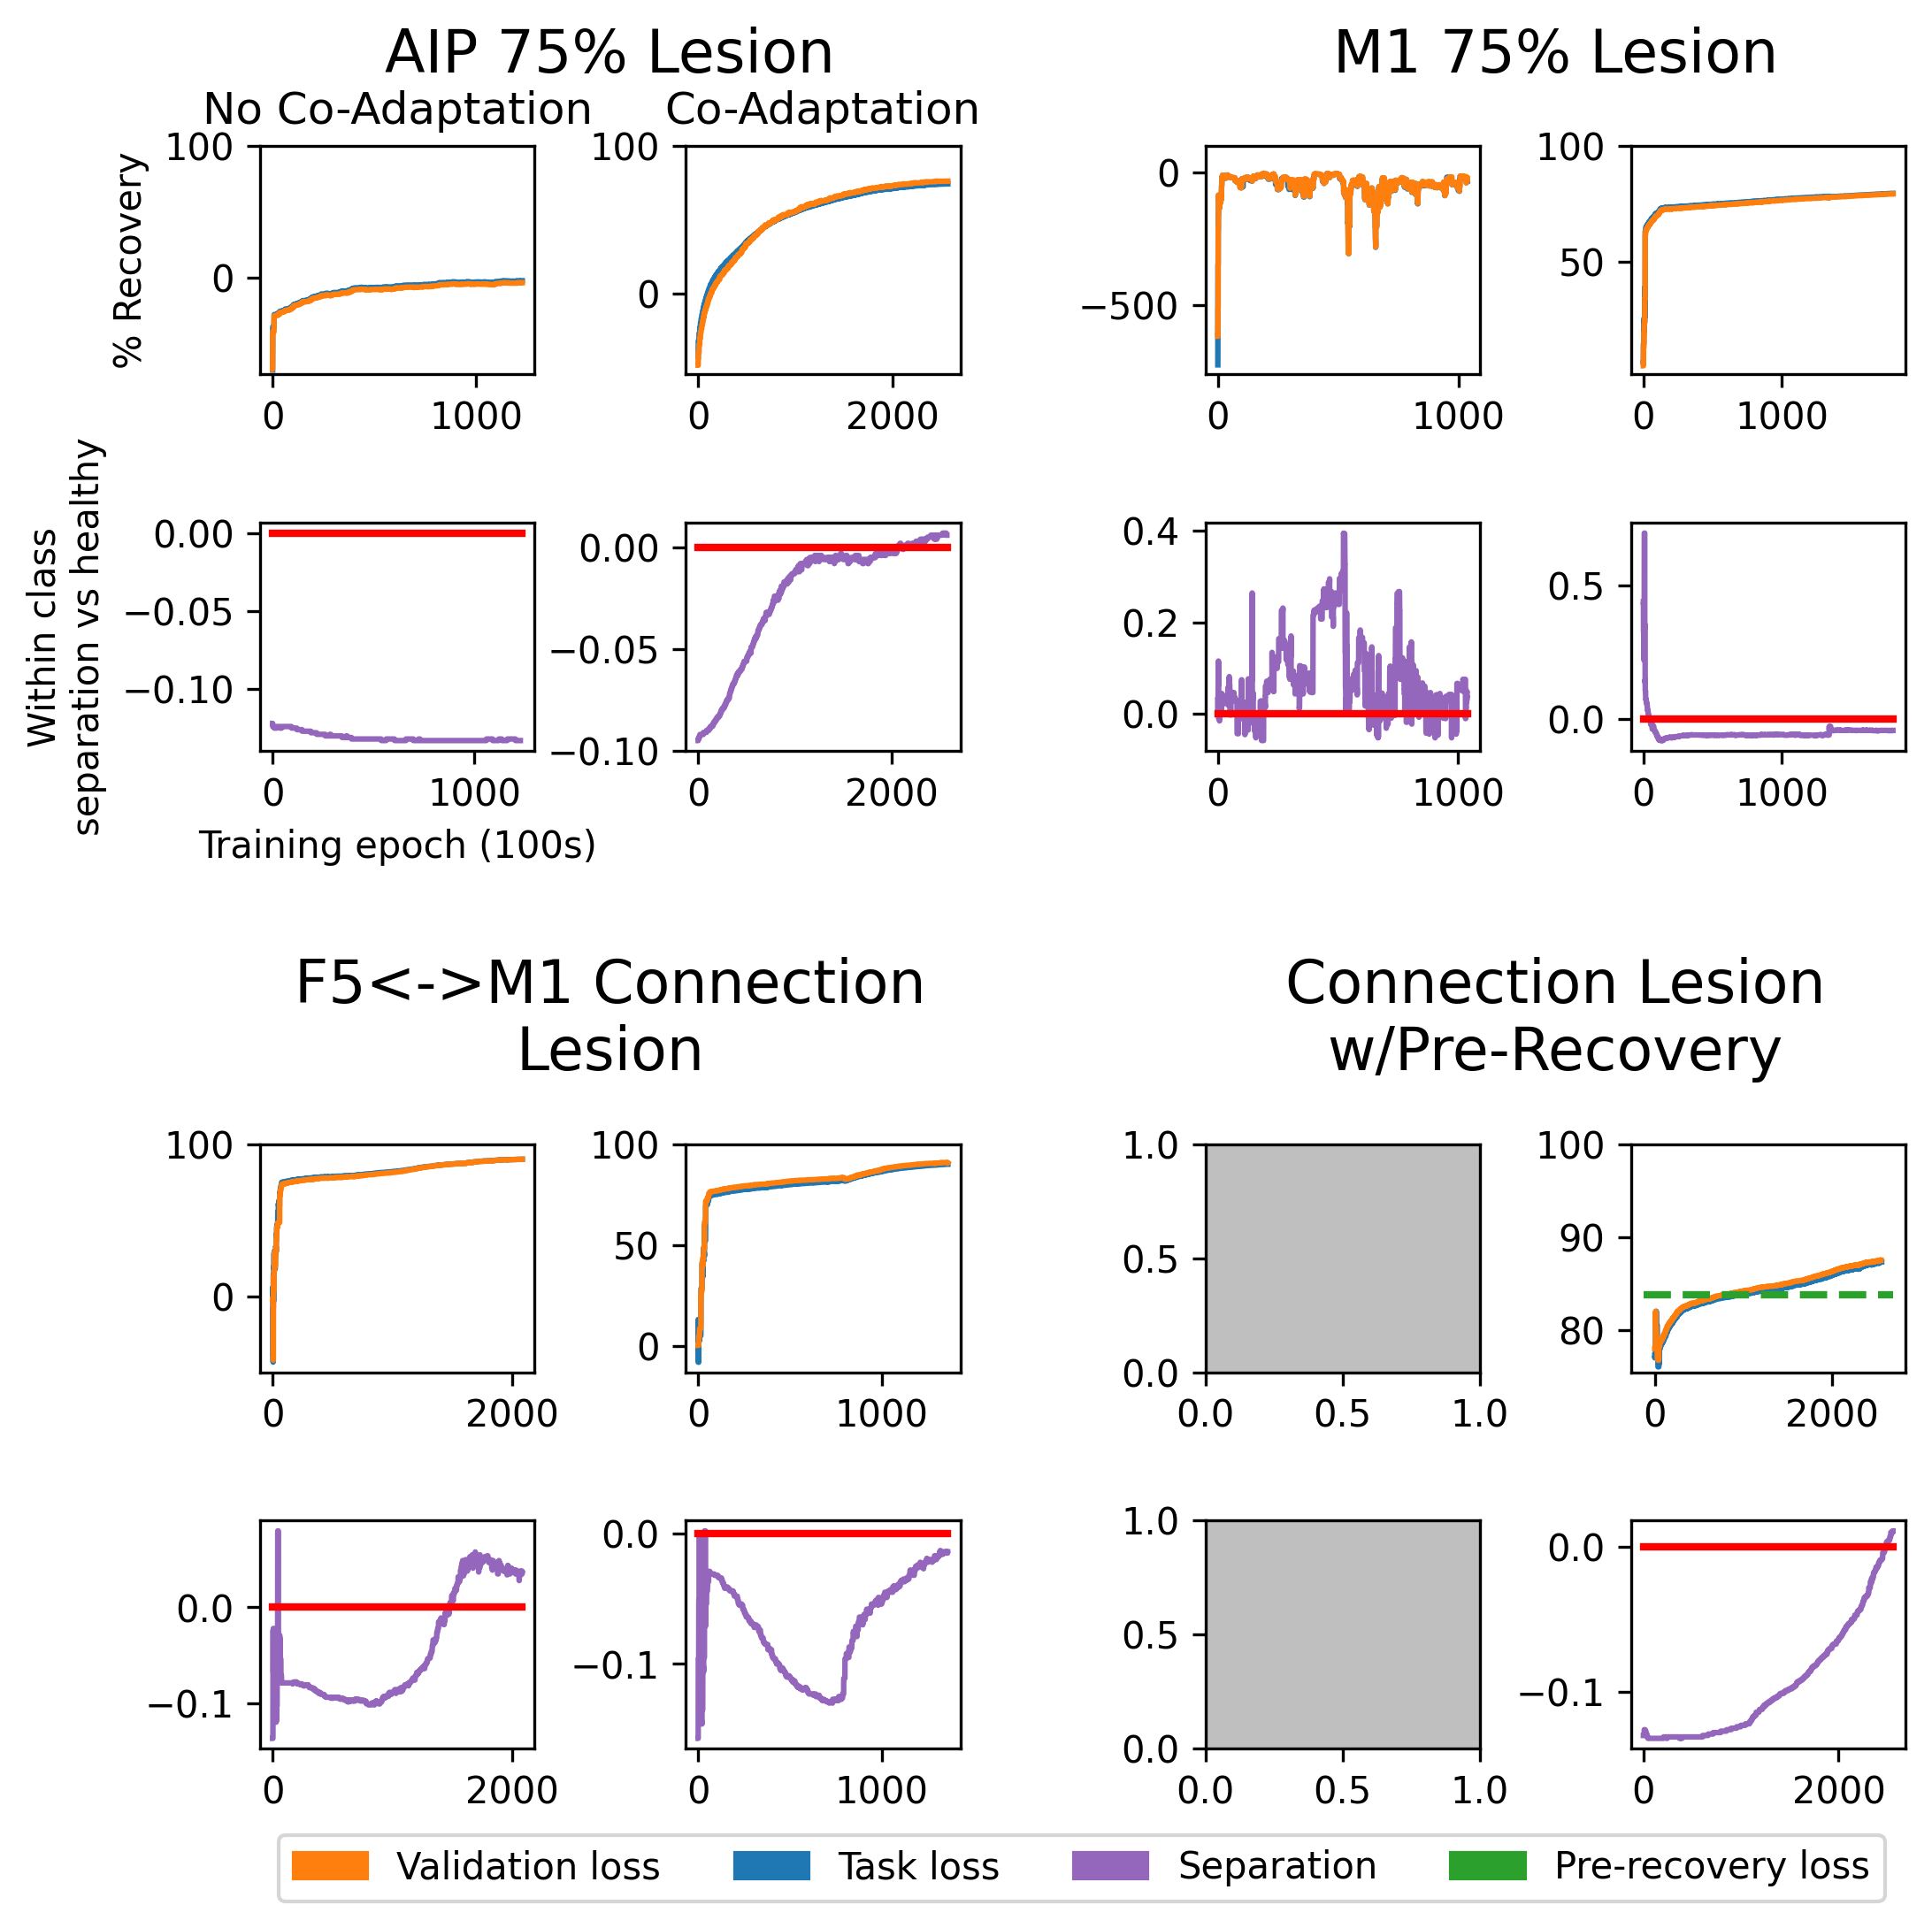
\includegraphics[width=\textwidth]{training_results.png}
\caption{Loss and class separation vs training epoch}
\centering
\label{fig:results}
\end{figure}

TODO: table of raw healthy vs lesioned vs recovered vs pct recovered

With each experiment, we track two metrics to characterize the learning progress. First, we
track the task loss, which is an MSE loss that measures the co-processor's ability to restore
movement towards the target trajectory. We characterize that measure in terms of its percent
difference from lesioned and healthy performances.

Second, we measure the degree to which the co-processor's solution successfully
differentiates object classes. We measure the ratio of within-class and total variation,
and compare that to the healthy network. Our separation metric $S$ is defined as:

\begin{equation}
	S = \frac{\sigma_{a}}{\sigma_{w}} - \frac{\sigma_{a,h}}{\sigma_{w,h}}
\end{equation}

where $\sigma$ measures the mean variation, across time, and across all data points in
a given sample. $\sigma_{a}$ is the total variation of a dataset, and $\sigma_{w}$
is the average of the within-class variations. The $h$ indicates the healthy
metric. An $S$ value of 0.0 indicates that the grasps for the various object classes
vary to the same degree as the healthy network.

This metric $S$ allows us to differentiate overall task performance improvement
and the ability of the co-processor to condition the grasp based on visual information.
The structure of the delayed reach-to-grasp task can be learned by the co-processor,
i.e. to hold muscle velocities to 0.0 for the initial part of each trial, without it
also learning to differentiate the various object shapes from the brain observations.
$S$ is our metric for differentiating those two co-processor behaviors.

\subsection{Experiment 1: AIP 75\% lesion}
This experiment measures the effect of a loss of task representation neural
machinery on the ability of the co-processor to succeed. In the non-coadaptive
version of this experiment, the loss of neurons involved in encoding the
visual inputs results in the simulated brain being unable to condition its
grasp for the object shape. Likewise, the co-processor doesn't have sufficient
information to improve performance. The lesioned circuit largely 

In the co-adaptive case, 

See Fig. \ref{fig:results}.

\subsection{Experiment 2: M1 75\% lesion}
\subsection{Experiment 3: F5 and M1 connectivity lesion}
\subsection{Experiment 4: M1 lesion with pre-recovery}

TODO: summary of conclusions that will go here:

TODO:
* AIP + coadaptation shows that we can adapt to changes in the input mappings.
* M1 + coadaptation shows we can adapt to changes in the output mappings
* Connection lesion shows we can act as a bridge

\begin{itemize}
	\item Task performance improves drastically. In all cases, performance is still improving slowly when I stop the simulation.
		\begin{itemize}
			\item 90\% on connection lesion, both with and without co-adaptation
			\item M1 50\%: 81\% recovery with and without co-adpation. The co-processor is having trouble finding a better solution than this, due to loss in brain functionality. Increasing the rate of brain co-adaptation may show a better solution.
			\item AIP 50\%: 53\% recovery w/co-adaptation so far; still running. The loss was very low to start with, and recovery depends heavily on co-adaptation, so training is slow. Without co-adaptation, the co-processor cannot learn well, because too much encoding machinery is lost.
			\item Waiting on pre-recovery result. Unclear if the co-processor will help or not.
		\end{itemize}
	\item Initially, performance improves orders of magnitude more quickly than later. 50-75\% recovery during this phase. This appears to be the co-processor learning the task structure (e.g. not to move the hand until after the hold signal is lifted).
	\item Fine tuning takes a far longer time
	\item This may have some connection to object class separation; show class sep metric side-by-side. (I have the data in hand, but haven't tried to correlate it to recovery yet).
	\item Training efficiency analysis. The majority of epochs (80\%; depends on experiment type) are EN training epochs, so most efficiency gains will be there.
	\item Can co-adapt with the brain, as it changes
	\item Compare co-adaptive case vs not. Some tasks will be impossible to accomplish without the two cooperating, if enough cortex has been lost. (waiting for new results to confirm)
	\item Show pre-recovery results; co-processor will hopefully improve beyond what recovery can achieve. Initial result: the co-adaptive case found a better solution. The co-processor couldn't improve yet on the pre-recovery case. The solution it found was (basically) to ignore the inputs.
\end{itemize}

\section{Discussion and Future Work}
\label{sec:discussion}

We present here a first-of-its-kind demonstration of a novel design for neural co-processors,
allowing for an AI agent to learn neural stimulation policies that improve a user's performance
of an external task. The design revolves around the use of a stimulation model for training the
agent, providing a proxy to the true function mapping stimulation and neural activity
to task performance. We base our demonstration on a simulation of a neural circuit engaged in
an external grasping task.

Our co-processor design adapts well to a variety of simulated lesion types, reducing task loss
50-90\% across our various experiments. To work this well, the co-processor needed to adapt to
the long-running dynamics of the stimulated network, as well as the long-running effects of
stimulation. In some experiments we required it to additionally adapt to non-stationarity in
the neural circuit, which was actively changing at the same time the co-processor was learning.
It achieved that as well, co-adapting with the simulated brain to improve external task
performance. Finally, it adapted to a simulated brain which had already undergone some amount of
lesion recovery. In that case, the co-processor successfully identified the information upstream
from the lesion which was necessary to stimulate the motor cortex downstream.

Clearly, we need to discuss carefully what can and cannot be inferred from simulation studies
such as these. As in Dura-Bernal \cite{bernal.sim}, we note that our simulation differs
drastically from an organic brain, both in scale and structure. Today, predicting long-running
neural responses to stimulation remains a difficult problem, implying targeted neural control
is also difficult. Even moreso, identifying the neural correlates of complex task success
remains largely out of reach \cite{khanna.openloop}. What, then, does our simulation provide us?

Abstractly, the co-processor lends itself to any closed-loop neural stimulation problem
where a relevant stimulation model can be identified. There are many lower dimensional problems
today which we address with far simpler stimulation regimes than would be necessary for
e.g. remediating the symptoms of a stroke. In some applications, such as PD symptom relief,
stimulation is often parameterized by a single off-vs-on parameter, or a small handful of
parameters, where the key challenge is learning when to apply the stimulation, and
its shape and power. Our simulation demonstrates the ability of our training method to adapt to
higher dimensional problems than these, where additionally the long-running effects of
stimulation on the intended figure-of-merit must be modeled. These properties together
suggest it may be useful in lower dimensional problems where a stimulation model can be
estimated, and stimulation parameters can be tied to the target objective.

Our future work will include a reinforcement learning (RL) approach, where the co-processor
explicitly learns when to apply stimulation, in addition to parameterizing it. Its target
objective involves not only symptom relief, but also minimizing energy use. In this approach,
our CPN and EN may correspond to the Actor and Critic portions of an Actor-Critic model
for example. Here, the Critic would learn to value symptom relief, while attaching a cost
to stimulation, thus incentivizing an energy efficient approach.

One challenge remaining with our current co-processor design is training effiency.
On the whole, the co-processor quickly improved task performance, but required orders of
magnitude more training examples to achieve its highest levels of performance. Even
moderate amounts of recovery may be valuable to a user, but nevertheless we consider
training efficiency to remain a problem. Due to limits on patient fatigue, time, implant
battery life, and other concerns, it is not plausible to expect a learning algorithm
to have access to unlimited amounts of training data. As a result, it is necessary to
make efficient use of the data we can acquire. We believe there exist at least three
mitigations for that:

\begin{itemize}
	\item Retraining an existing EN, rather than regularly creating a new one. As
	      mentioned above, we encountered difficulty with this approach, but it remains
	      to be seen if this is a fundamental problem with our training method, rather
	      than a peculiarity of our simulation. Also, it remains unclear if a solution
	      for our simulation exists as well, which we've simply yet to identify. This
	      remains a future area of inquiry.
	\item Making better use of what data we acquire. In this initial simulation we do
	      not retain data beyond the present training epoch. In practice, we can likely
	      retain training data for some time window. Non-stationarity requires us to
	      regularly discard or discount data as it ages. However, in practice, training
	      epochs operate on the order of seconds, suggesting that data can be retained
	      and reused for multiple epochs. The `speed' of non-stationarity compared to
	      the co-processor's learning therefore must be an area of future research.
	\item Matching the dimensionality of the stimulation and observations
	      to the amount of available data. If one chooses a stimulation regime with
	      a small number of controllable parameters, where nevertheless task improvement
	      from the stimulation is possible, that allows for a simpler co-processor which
	      will likely require less training data.
\end{itemize}

Having now demonstrated our method on a higher dimensional problem, we will next demonstrate
it on a lower dimensional problem, one which is likely to transfer more readily to
an \textit{in vivo} trial. We hypothesize that this co-processor model will transition well
to applications in PD, or essential tremor (ET). In Castaño-Candamil et al. \cite{castano.pd},
we see an ML-based approach to closed-loop stimulation for ET relief. Here, a simple learning
model extracts neural markers (NMs) from a human patient's M1 cortex. It uses those to
condition DBS stimulation parameters. The stimulation controller adapts to non-stationarity
of the mapping between NMs and optimal control, which is necessary due to the sensitivity
of NMs to context (e.g. sitting or standing). The co-processor model is likely to
transition well to such an application, where it may provide additional energy savings
or reduction of stimulation side-effects. In that case, it will attempt to extract neural
markers appropriate for each context, to detect transitions in context, and to apply
optimal stimulation.

\section{Conclusion}
We have demonstrated a general framework for training a closed-loop neural stimulator,
called a ``neural co-processor''. We outlined one specific co-processor design, and
outlined an approach to training it using supervised learning. In simulation it
successfully learned to alleviate some of the effects of a brain lesion. To do so, it
needed to co-adapt to the simulated brain, which exhibited non-stationarity. Additionally,
it needed to learn long-running effects of the stimulation it learned to apply. Because of
these properites, the co-processor approach likely generalizes well to a wide range of
clinical applications where closed-loop neural stimulation is appropriate.

\section{Acknowledgements}
TODO: funding sources

The author would like to thank the following for discussions and insights related to
the present topic:
\begin{itemize}
	\item Karunesh Ganguly, UC San Francisco
	\item Priya Khanna, UC San Francisco
	\item Anca Dragan, UC Berkeley
	\item Justin Ong, University of Washington
	\item Luciano De La Iglesia, University of Washington
\end{itemize}

\section{References}
\bibliographystyle{iopart-num}
\bibliography{refs}
\end{document}

